\section{Numerical experiments}\label{sec:numerical_experiments}
This section analyzes the performance of \methodAcronymROMs\ leveraging \spatialAcronym\ trial subspaces on two benchmark problems: the Sod shock tube and compressible flow in a cavity. In each experiment, \methodAcronym\ is compared to the Galerkin and LSPG ROMs. The purpose of the numerical experiments is to assess the impact of minimizing the residual over an arbitrarily sized time window on the solution accuracy. We additionally assess the impact of the time step and time scheme on \methodAcronym. In both experiments, the spatial basis is equivalent for each time window, e.g., $\basisspaceArg{n} \equiv \basisspace$, $n=1,\ldots,\nslabs$. It is also noted that both experiments are designed to test the \textit{reproductive} ability of the ROMs. Future state prediction and prediction at new parameter instances are not considered as these problems introduce factors that confound the solution accuracy with the solution methodology (e.g., accuracy of the basis). 
 
\subsection{Sod shock tube}
We first consider reduced-order models of the Sod shock tube problem. The system is governed by the compressible Euler equations in one dimension, 
\begin{equation}\label{eq:euler_1D}
    \frac{\partial \boldsymbol u}{\partial t} + \frac{\partial \boldsymbol F}{\partial \mathsf{x}} = 0, \quad
    \boldsymbol u= 
    \begin{Bmatrix} \rho \\ \rho u \\ \rho E \end{Bmatrix}, \quad 
    \boldsymbol F = \begin{Bmatrix} \rho u \\ \rho u^2 + p \\  u(\rho E + p) \end{Bmatrix},
\end{equation}
where $\boldsymbol u : \Omega \times [0,T] \rightarrow \RR{3}$ comprise the density, x-momentum, and total energy, $\mathsf{x} \in \Omega \defeq  [0,1]$ is the spatial domain, and 
$T = 1$ the final time. 
The problem setup is given by the initial conditions

\begin{equation*}
\rho = 
\begin{cases} 
      1 & \mathsf{x}\leq 0.5 \\
      0.125 & \mathsf{x} > 0.5 
   \end{cases},
\qquad
p = 
\begin{cases} 
      1 & \mathsf{x}\leq 0.5 \\
      0.1 & \mathsf{x} > 0.5 
   \end{cases},
\qquad
u = 
\begin{cases} 
      0 & \mathsf{x}\leq 0.5 \\
      0 & \mathsf{x} > 0.5 
   \end{cases},
\end{equation*}
along with reflecting boundary conditions at $\mathsf{x}=0$ and $\mathsf{x}=1$. 

\subsubsection{Description of FOM and generation of \spatialAcronym\ trial subspace}\label{sec:sod_fom}
The 1D compressible Euler equations are solved using a finite volume method. The domain is partitioned into 500 cells of uniform width. The finite volume method uses the Rusanov flux~\cite{rusanov} at the cell interfaces. The FOM uses the Crank--Nicolson (CN) scheme, which is a linear multistep method defined by the coefficients $\alpha_0 = 1,\alpha_1 = -1, \beta_0 = \beta_1 = 1/2$, for temporal integration. The FOM is evolved for $t \in [0.0,1.0]$ at a time-step of $\Delta t = 0.002$. The \spatialAcronym\ trial subspace is constructed by executing Algorithm~\ref{alg:pod} with inputs $N_{\text{skip}}=2, \stateIntercept = \bz, K=46 $. The resulting trial subspace corresponds to an energy criterion of $99.99\%$.
%  The solution is saved every other time-step, resulting in 500 solutions snapshots. These snapshots are used to generate a trial basis for the reduced-order models through POD. The trial basis is selected to be of dimension $K = 46$, which corresponds to a $99.99\%$ energy criterion. No affine transformation is used in the construction of the trial subspace, i.e., $\stateIntercept = \bz$.

\subsubsection{Description of reduced-order models}
We consider reduced-order models based on the Galerkin, LSPG, and \methodAcronym\ approach. No hyper-reduction is considered 
in this example, i.e., $\stweightingMatArg{n} = \mathbf{I}$, $n=1,\ldots,\nslabs$. Details on the implementation of the 
different reduced-order models is as follows:
\begin{itemize}
\item \textit{Galerkin ROM}: The Galerkin ROM is obtained through Galerkin projection of the FOM. The Galerkin ROM is evolved in time with the CN time scheme at 
a constant time step of $ \Delta t = 0.002$.

\item \textit{LSPG ROM:} The LSPG ROM is built on top of the FOM discretization leveraging the CN time scheme as previously described. Unless noted otherwise, the LSPG ROM uses a constant time step of $\Delta t = 0.002$. The nonlinear least-squares problem arising at each time instance is solved via the Gauss--Newton method. The linear least-squares problems arising at each Gauss--Newton iteration are solved via the normal equations. All Jacobians are computed via automatic differentiation~\cite{adolc}. The Gauss--Newton algorithm is deemed converged when the gradient norm is lower than $10^{-4}$. 
\item \textit{\methodAcronymROM:} \methodAcronymROMs\ are solved via the direct and indirect methods with two different time-stepping schemes: 
\begin{itemize}
\item Direct method: We consider \methodAcronymROMs\ solved via the direct method for both the same CN discretization employed in the FOM and LSPG, as well as for the second-order explicit Adams Bashforth (AB2) discretization using a constant time step of $\Delta t = 0.0005$. The nonlinear least-squares problem 
arising over each window is solved via the Gauss--Newton method. The linear least-squares problems arising at each Gauss--Newton iteration is solved via the normal equations. All Jacobians are again computed via automatic differentiation, and the Gauss--Newton algorithm is deemed converged when the gradient norm is lower than $10^{-4}$ (i.e., we use the parameter $\epsilon = 10^{-4}$ in Algorithm~\ref{alg:colloc_gn}). Critically, it is noted that the Jacobian 
matrix over a window is constructed by assembling local (dense) Jacobians. The global Jacobian over a single window is then stored in a compressed sparse row format. Uniform quadrature weights are used for evaluating the integral in~\eqref{eq:obj_gen_slab}. 

\item Indirect method: We consider two \methodAcronymROMs\ solved via the indirect method. The first uses the same CN discretization at at time step of $\Delta t = 0.002$, while the second uses the AB2 discretization using a time step of $\Delta t = 0.0005$. The coupled two-point boundary 
problem is solved via the forward--backward sweep method. The action of the Jacobian transpose on vectors is computed via automatic differentiation. We use parameters $\epsilon = 10^{-6}$, $\fbsmGrowth = 1.1$, and $\fbsmDecay=2$ in Algorithm~\ref{alg:st_iter}. 
\end{itemize}
\end{itemize}

%We explore the evaluation of the \methodAcronym\ ROM using both indirect and direct solution methodologies. 
%\subsubsection{Indirect Method}
%The indirect \methodAcronym-ROM solves the coupled boundary value problem using the Forward-Backward Sweep Method (FBSM) described in Section~\ref{sec:fbsm}. A secondd-order collocation method with a time-step size of $\Delta t = 0.002$ and with collocation points placed at the Lobatto points is used for discretization of both the forward and backwards problems. The action of the Jacobian transpose on the residual and adjoint state required for the backwards problem is computed through automatic differentiation~\cite{adolc,pyadolc}. 
%
%\subsubsection{Direct Method}
%The direct \methodAcronym-ROM uses the same second-order collocation method with uniformly distributed collocation points for temporal discretization of both the state 
%and integrand. The resulting least-squares problem is solved using the Gauss-Newton method. The inner Gauss-Newton iterations are solved using the conjugate gradient 
%method preconditioned by the inverse approximate Hessian about the initial guess. 



\subsubsection{Numerical results}
The impact of the window size on \methodAcronymROMs\ is first assessed. We consider a set of \methodAcronymROMs\ that minimize the residual over windows of constant size 
$\DeltaSlabArg{n} \equiv \DeltaSlabArg{} =  .002$, $0.004$ ,$0.008$, $0.02$, $0.04$, $0.10$, $0.20$, $1.0$. We additionally consider the standard Galerkin and LSPG ROMs. We first show results for \methodAcronymROMs\ using the direct method with CN time discretization; a comparison of different time-marching methods and direct/indirect solution techniques will be provided later in this section. 
First, Figure~\ref{fig:sod_density} presents the density solutions predicted by the various ROMs at $t = 0.5$ and $1.0$. Figure~\ref{fig:sod_xt} shows 
$x-t$ diagrams for the same density solutions. From Figures~\ref{fig:sod_density} and~\ref{fig:sod_xt}, it is observed that the LSPG and Galerkin ROMs accurately characterize 
the system: they correctly track the shock location, expansion waves, etc. We observe both predictions, however, to be highly oscillatory. These oscillations are 
not physical and can lead to numerical blowup; e.g., due to negative pressure. We observe the \methodAcronymROMs\ to produce less oscillatory solutions than both 
the Galerkin and LSPG ROMs. Critically, we see that the solution becomes less oscillatory as the window size over which the residual is minimized grows. The solution displays no oscillations when the residual is minimized over the entire space--time domain. 

%The impact of the window-size over which the residual is minimized on the ROM solution is first examined. To this end, reduced-order models that minimize the residual over windows of size $\Delta \tau = \Delta t \times [2,5,10,20,50,100,200,1000,2000]$ are considered. Figure~\ref{fig:xtrho} summarizes the performance of the various reduced-order models. Figure~\ref{fig:sod_error_a} shows the integrated $L^2$ state error relative to the Galerkin ROM. Figure~\ref{fig:sod_error_b} shows the space-time residual of the various reduced-order models as measured realitive to the full-order model. In Figure~\ref{fig:sod_error_a}, it is seen that the optimal ROM as measured by the integrated $L^2$ state error occurs at an intermediate window size. This result is perhaps somewhat surprising as one may expect the optimal $L^2$ error to occur when the window size spans the entire temporal domain, in which case the total space-time residual is minimized. As is evident from Figure~\ref{fig:sod_error_a}, however, a lower space-time residual does not necesarily imply a lower error. Figure~\ref{fig:sod_error_b} shows the total integrated space-time residual of the various ROMs as measured with respect to the projected full-order model solution. Increasing the window-size over which the residual is minimized leads to a lower over-all space-time residual. Further, when the residual is minimized over the entire space-time domain ($\Delta \tau =2000$), it is lower than that of the projected full-order model. This numerical evidence supports the theoretical error analysis presented in Section~\ref{sec:error}. In this example, the global space-time residual is lower than that of the projected full-order model for $\Delta \tau > 0.01$.  
%
%Figure~\ref{fig:sod_density} shows density profiles predicted by the CWST-LSPG ROM at two different time instances along with integrated total variation of the solution as measured with respect to the full-order model. It is observed that, as the window size over which the residual is being minimized grows, the solution becomes more smooth. This is measured quantitatively by the total variation of the solution, which decreases monotonically as the window size grows. Next, Figure~\ref{fig:xtrho} shows $x-t$ diagrams for the density variable for the various reduced-order models. It is again seen that, as $\Delta \tau$ grows, the solution becomes more smooth. The increased smoothness comes at the tradeoff that the shock profiles become more smeared. 
%
%Lastly, Figure~\ref{fig:sod_walltime} shows the wall-time of the CWST-LSPG ROM as a function of window-size. The cost is measured with respect to the Galerkin ROM. Two main observations are made. First, the cost of the CWST-LSPG ROM increases as the window size grows. This increased cost is because, as the window size grows, more iterations of the forward and backwards problems are required to converge the solution. While a more sophisticated solution methodology may help mitigate this increased cost, the trends are expected to say the same. The second observation is that the CWST-LSPG ROM is significantly more expensive than the standard Galerkin ROM. As discussed in Section~\ref{sec:implement}, this increased cost is due to the need to iteratively solve the two-point boundary value problem. 
\begin{figure}
\begin{center}
\begin{subfigure}[t]{0.45\textwidth}
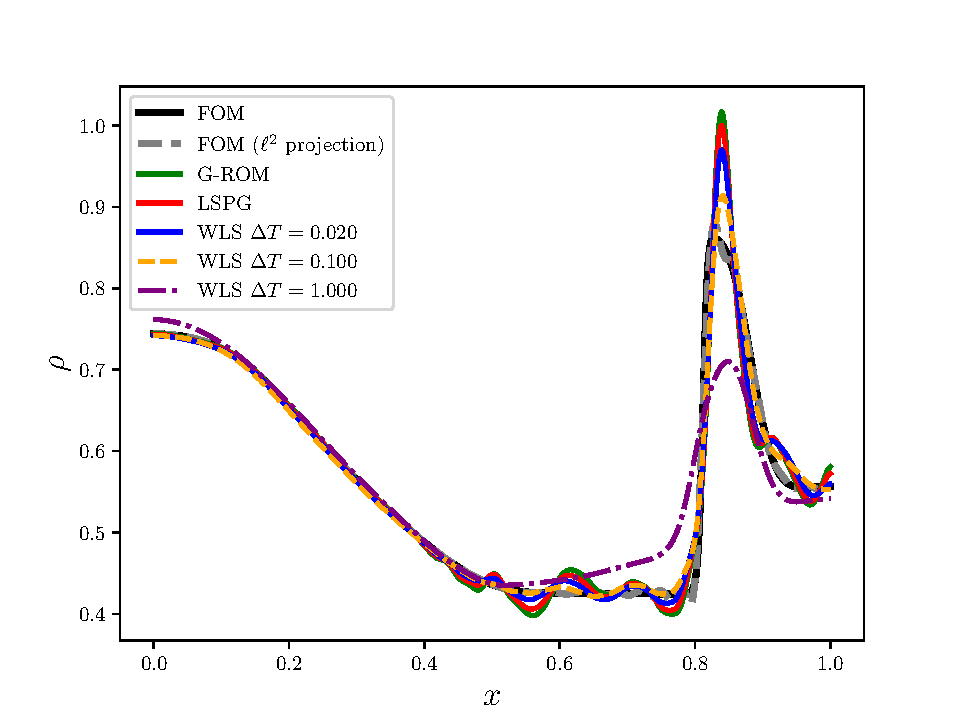
\includegraphics[width=1.\linewidth]{figs/sod/rho_t05_compare.pdf}
\caption{$t=0.5$}
\end{subfigure}
\begin{subfigure}[t]{0.45\textwidth}
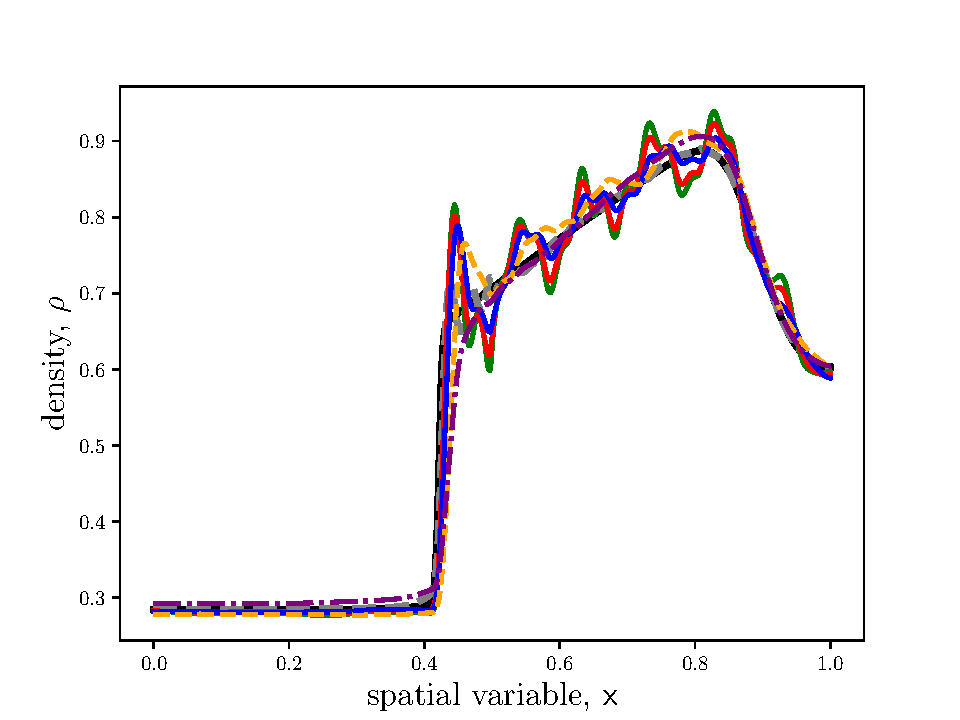
\includegraphics[width=1.\linewidth]{figs/sod/rho_t1_compare.pdf}
\caption{$t=1$}
\end{subfigure}
\caption{Density profiles at various time instances.}
\label{fig:sod_density}
\end{center}
\end{figure}


\begin{figure}
\begin{center}
\begin{subfigure}[t]{0.48\textwidth}
\includegraphics[width=1.\linewidth]{figs/sod/xt_fom.pdf}
\caption{Full-order model}
\end{subfigure}
\begin{subfigure}[t]{0.48\textwidth}
\includegraphics[width=1.\linewidth]{figs/sod/xt_grom.pdf}
\caption{G-ROM}
\end{subfigure}
\begin{subfigure}[t]{0.48\textwidth}
\includegraphics[width=1.\linewidth]{figs/sod/xt_lspg.pdf}
\caption{LSPG}
\end{subfigure}
\begin{subfigure}[t]{0.48\textwidth}
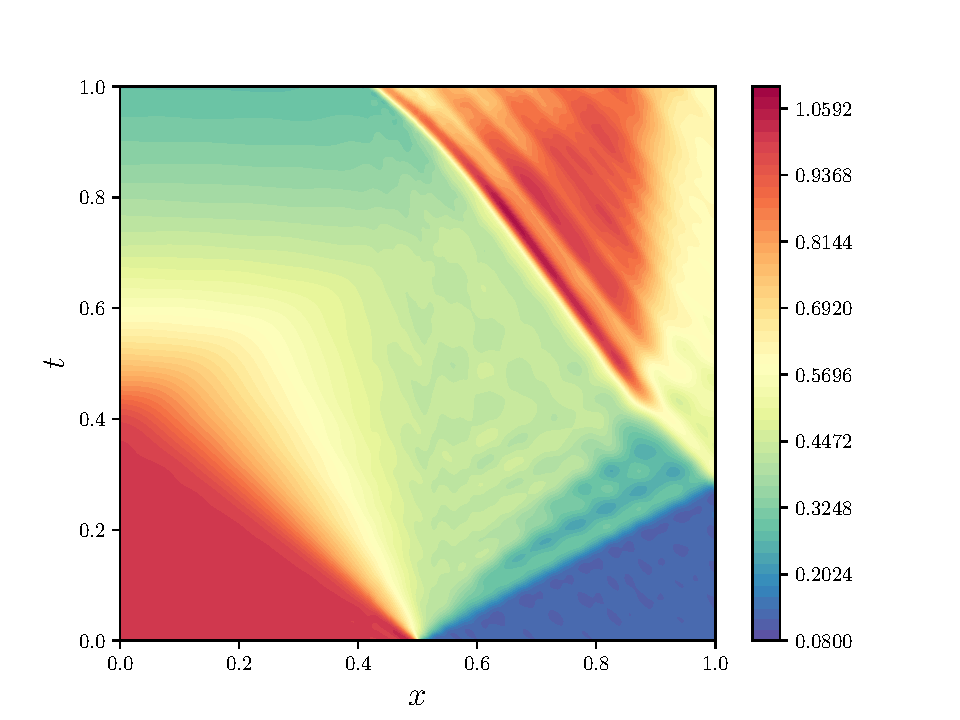
\includegraphics[width=1.\linewidth]{figs/sod/xt_w1.pdf}
\caption{\methodAcronym: $\DeltaSlabArg{}= 0.002$}
\end{subfigure}
\begin{subfigure}[t]{0.48\textwidth}
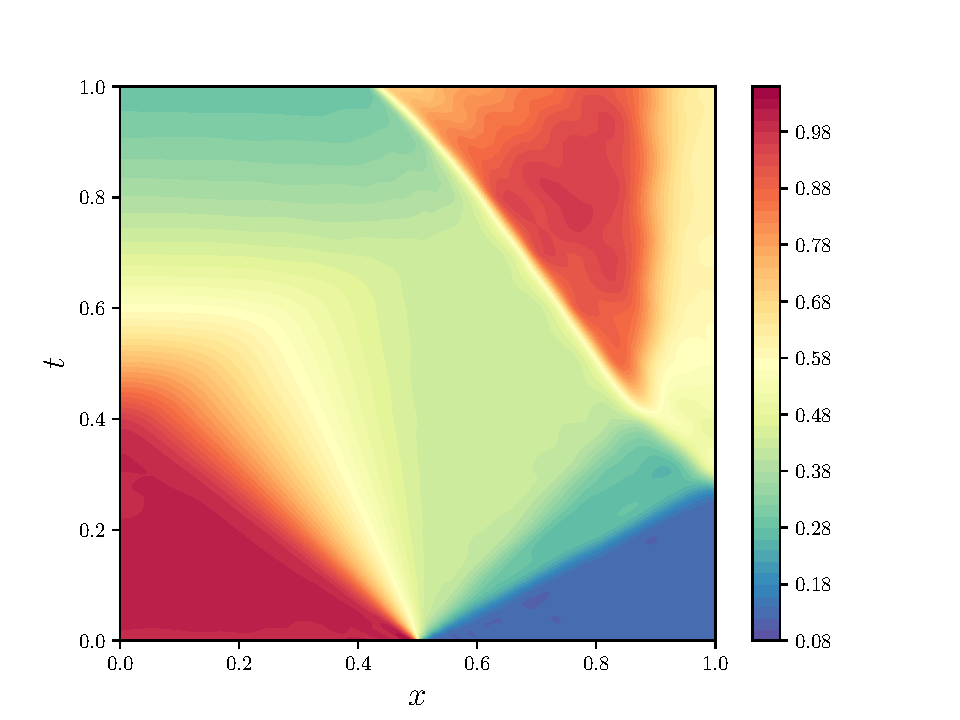
\includegraphics[width=1.\linewidth]{figs/sod/xt_w50.pdf}
\caption{\methodAcronym: $\DeltaSlabArg{} = 0.1$}
\end{subfigure}
\begin{subfigure}[t]{0.48\textwidth}
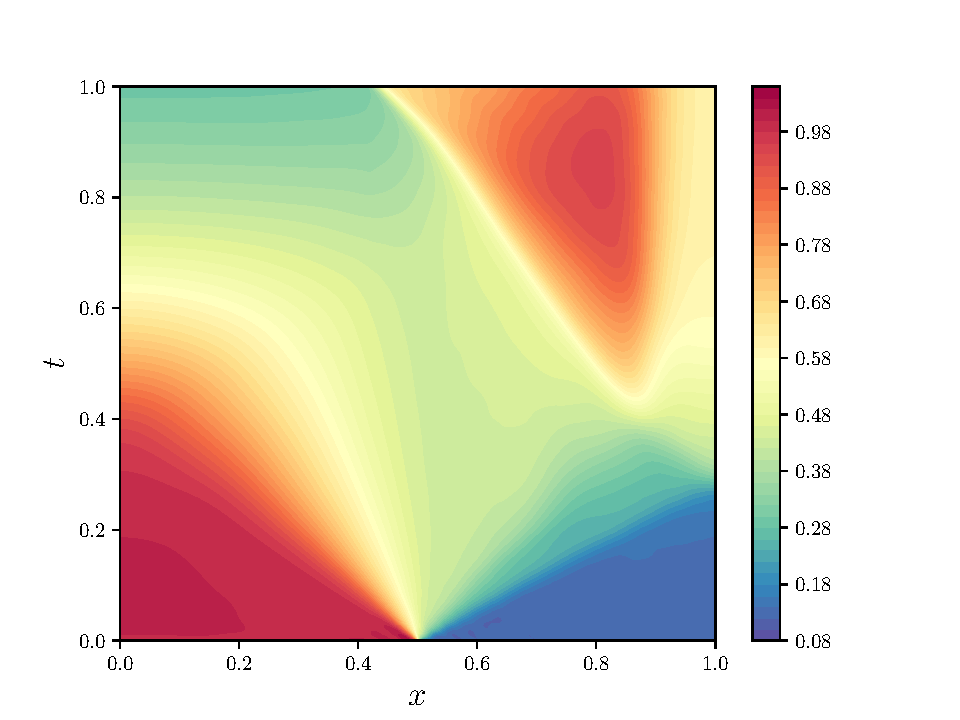
\includegraphics[width=1.\linewidth]{figs/sod/xt_w500.pdf}
\caption{\methodAcronym: $\DeltaSlabArg{} = 1.0$}
\end{subfigure}
\caption{$x-t$ diagrams for the density fields as predicted by the FOM, G-ROM, LSPG-ROM, and \methodAcronymROMs.}
\label{fig:sod_xt}
\end{center}
\end{figure}

Next, Figure~\ref{fig:sod_error} shows space--time (i.e., integrated) state errors and the objective function~\eqref{eq:obj} (i.e., the space--time residual norm) over $t \in [0,1]$ for the various ROMs. Most notably, we observe 
that increasing the window size over which the residual is minimized does \textit{not} lead to a monotonic decrease in the space--time $\elltwo$  
error. Increasing the window size does lead to a monotonic decrease in the space--time residual, however. We additionally note that, although the space--time
$\elltwo$ error of 
the projected FOM solution is significantly lower than that of the various ROM solutions, the space--time residual norm of the projected FOM solution is \textit{higher} 
than all ROMs. Thus, although the projected FOM solution is more accurate in the $\elltwo$ norm, it does not satisfy the governing equations as well the ROM solutions. 

\begin{figure}
\begin{center}
\begin{subfigure}[t]{0.45\textwidth}
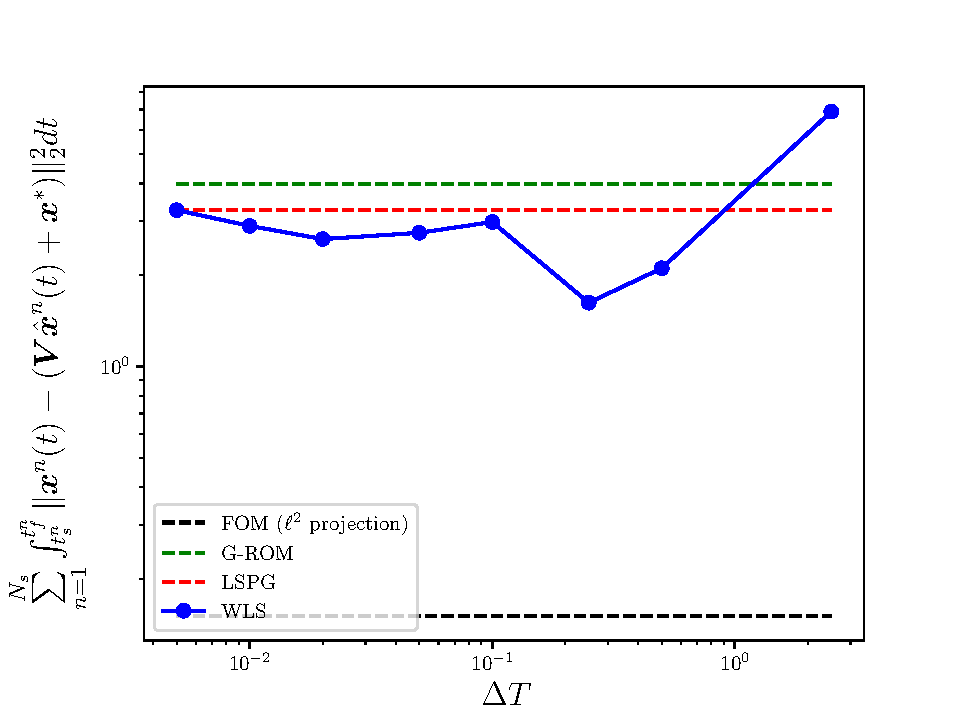
\includegraphics[width=1.\linewidth]{figs/sod/error_vs_window_compare.pdf}
\caption{Space--time $\elltwo$ error of various ROMs.}
\label{fig:sod_error_a}
\end{subfigure}
\begin{subfigure}[t]{0.45\textwidth}
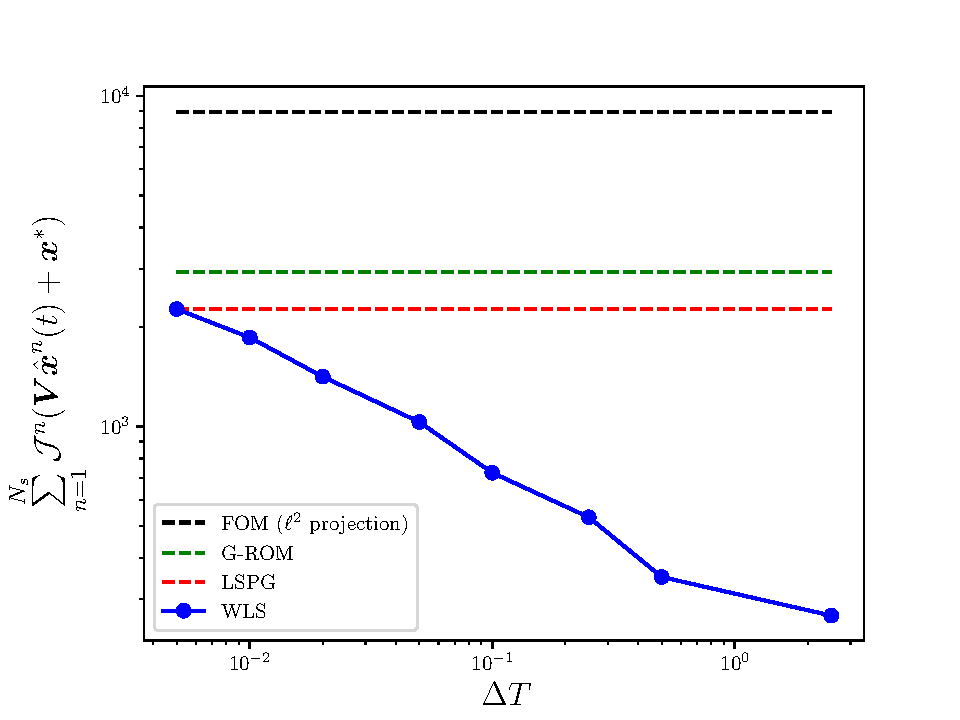
\includegraphics[width=1.\linewidth]{figs/sod/objective_vs_window_compare.pdf}
\caption{Integrated residual norm of various ROMs.} 
\label{fig:sod_error_b}
\end{subfigure}
\caption{Integrated performance metrics of the Galerkin, LSPG, and \methodAcronymROMs.  Note that the Galerkin and LSPG ROMs do not depend on the window size.} 
\label{fig:sod_error}
\end{center}
\end{figure}

We now examine the comparative performance of the direct and indirect solution techniques for the \methodAcronymROMs\ using various time discretization techniques. 
Figure~\ref{fig:sod_error_methods} 
shows the same space--time $\elltwo$ state errors and residual norms as in Figure~\ref{fig:sod_error}, but this time results are shown for 
the various \methodAcronymROMs. In both Figures~\ref{fig:sod_error_methods_a} and~\ref{fig:sod_error_methods_b}, we observe observed that the \methodAcronym\ method 
is relatively insensitive to the solution technique (direct vs indirect) and underlying discretization scheme, although some minor differences are observed.
In particular, ROMs using the second order explicit AB2 scheme with a time step of $\Delta t = 0.0005$ provide similar results to the 
ROMs using the second-order CN scheme at a time step of $\Delta t = 0.002$. All methods display similar dependence on the window size: the optimal space--time
$\elltwo$ state error occurs when the window size is $\DeltaSlabArg{} = 0.1$ and the residual decreases monotonically as the window size grows. 
\begin{figure}
\begin{center}
\begin{subfigure}[t]{0.45\textwidth}
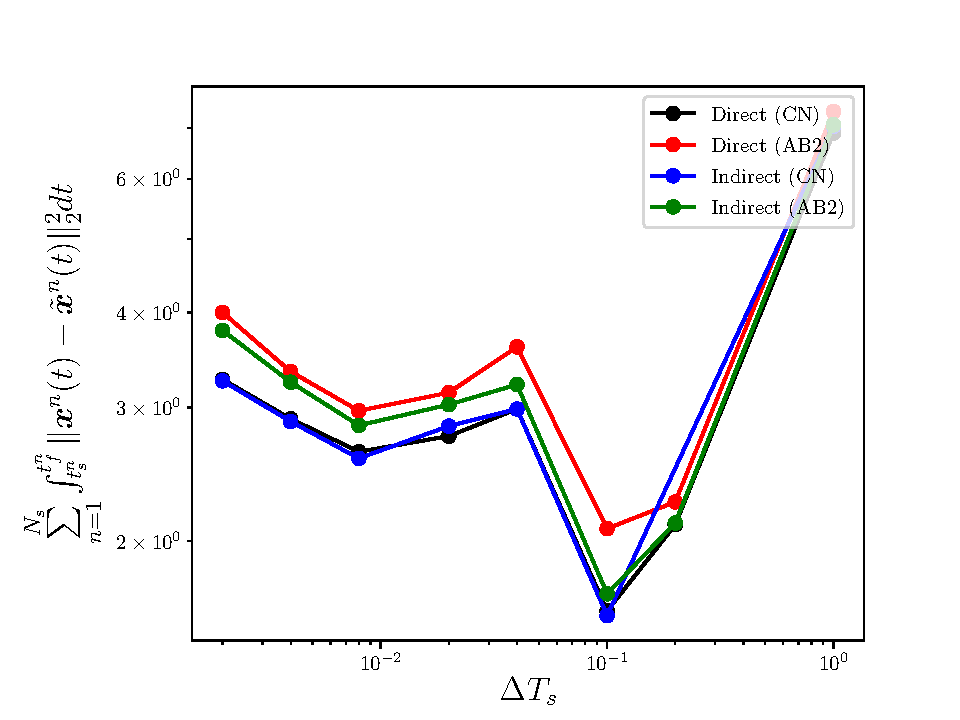
\includegraphics[width=1.\linewidth]{figs/sod/error_vs_window.pdf}
\caption{Integrated $\elltwo$ error of the \methodAcronymROMs.}
\label{fig:sod_error_methods_a}
\end{subfigure}
\begin{subfigure}[t]{0.45\textwidth}
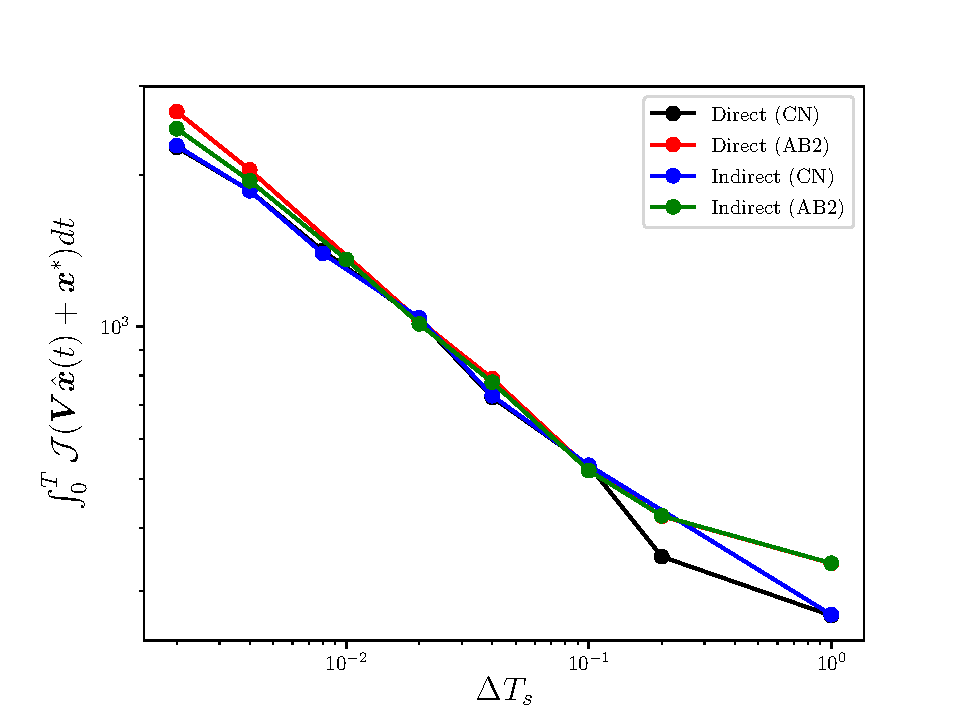
\includegraphics[width=1.\linewidth]{figs/sod/objective_vs_window.pdf}
\caption{Integrated residual norm of the \methodAcronymROMs.} 
\label{fig:sod_error_methods_b}
\end{subfigure}
\caption{Integrated performance metrics of various \methodAcronymROMs.} 
\label{fig:sod_error_methods}
\end{center}
\end{figure}


Next, Figure~\ref{fig:sod_walltime} provides the CPU wall-clock times for the various \methodAcronymROMs. The computational cost of all methods is seen to grow 
as the window size is increased. For indirect methods, this increase in cost is due to the fact that, as the window size 
grows, more iterations of the FBSM are required for convergence. For direct methods, the increase in cost is due to (1) the cost 
associated with forming and solving the normal equations at each Gauss--Newton iteration and (2) the increased number of 
Gauss--Newton iterations required for convergence. The cost of the FBSM method is observed to increase more rapidly 
than the direct methods. Encouragingly, \methodAcronymROMs\ based on the CN discretization
minimizing the full space--time residual (comprising 
500 time instances) only  
cost approximately one order of magnitude more than the case where the residual is minimized over a single time-step (i.e., LSPG). Also of interest is the 
fact that the direct method utilizing the AB2 time-discretization scheme costs only slightly more per a given window size than the direct method 
utilizing the CN time discretization. This is despite the fact that AB2 is evolved at a time step of $\Delta t = 0.0005$, while CN uses $\Delta t = 0.002$; thus 
AB2 contains 4 times more temporal degrees of freedom than CN.  Finally, we emphasize that the 
results presented here are presented for standard algorithms (e.g., Guass--Newton and the FBSM). As mentioned in 
Remarks~\ref{remark:gaussnewton} and~\ref{remark:fbsm}, we expect the computational cost 
of both the indirect and direct methods can be decreased through the use and/or development of 
algorithms tailored to the minimization problem. 


\begin{figure}
\begin{center}
\begin{subfigure}[t]{0.45\textwidth}
%\includegraphics[width=1.\linewidth]{/Users/ejparis/PyROM/pyrom/sod/postProcess_wv/error_vs_window.pdf}
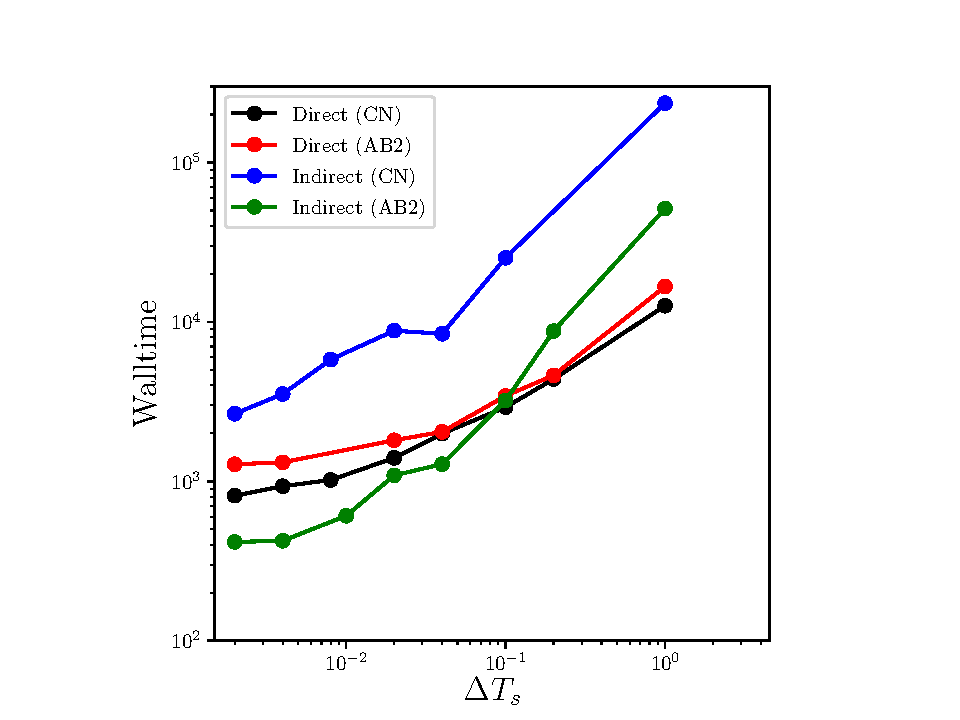
\includegraphics[width=1.\linewidth]{figs/sod/walltime_vs_window.pdf}
\label{fig:sod_error_a}
\end{subfigure}
\caption{Comparison of wall-clock times of the direct and indirect \methodAcronymROMs\ as a function of window size.} 
\label{fig:sod_walltime}
\end{center}
\end{figure}

Finally, we study the impact of the time step on the \methodAcronymROM\ results. We examine \methodAcronymROMs\ that use a
window size of $\Delta T = 0.1$, with time steps $\Delta t =$  $0.001$, $0.002$, $0.005$, $0.01$, $0.05$, $0.1$ (i.e.,  
$100$, $50$, $20$, $10$, $2$, and $1$ time-steps per window). We additionally 
consider LSPG ROMs leveraging the same set of time steps. To assess time step convergence, we compare results to a new full-order model, which is as described in Section~\ref{sec:sod_fom} but uses a fine time step of $\Delta t = 1e-4$. Figure~\ref{fig:time_step_study} shows the space--time $\elltwo$ error and residual norm  
of the various ROMs. We observe that both the space--time $\elltwo$ error and residual norm 
of the \methodAcronymROMs\ decrease and converge as the time step decreases. This is in direct contrast to the LSPG ROMs, in where both the $\elltwo$ 
space--time error and residual norm increase as the time step decreases. This result 
demonstrates that \methodAcronym\ overcomes the time-step dependence inherit to the LSPG approach. Lastly, Figure~\ref{fig:walltime_dtvar}
shows the relative wall-clock times of the \methodAcronymROMs\ with respect to the LSPG ROMs. It is seen that, for all time steps considered, the \methodAcronym-ROMs 
are less than 6x the cost LSPG; despite the window sizes comprising up to 100 time steps. 
\begin{figure}
\begin{center}
\begin{subfigure}[t]{0.45\textwidth}
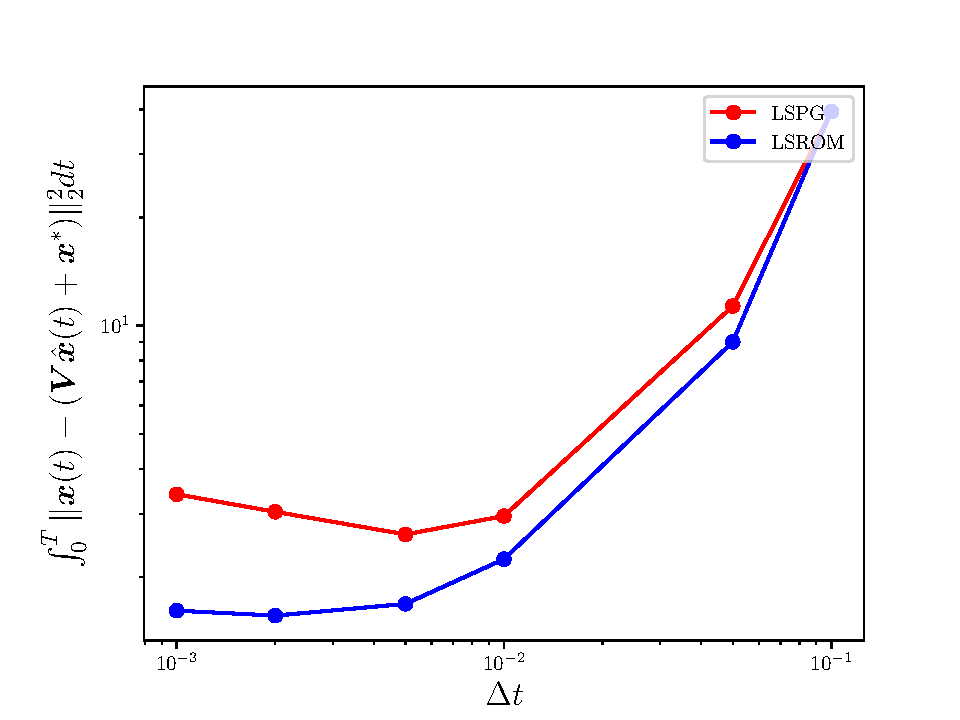
\includegraphics[width=1.\linewidth]{figs/sod/error_vs_window_dtvar.pdf}
\caption{Space--time $\elltwo$ error of the \methodAcronymROM.}
\label{fig:sod_error_methods_a}
\end{subfigure}
\begin{subfigure}[t]{0.45\textwidth}
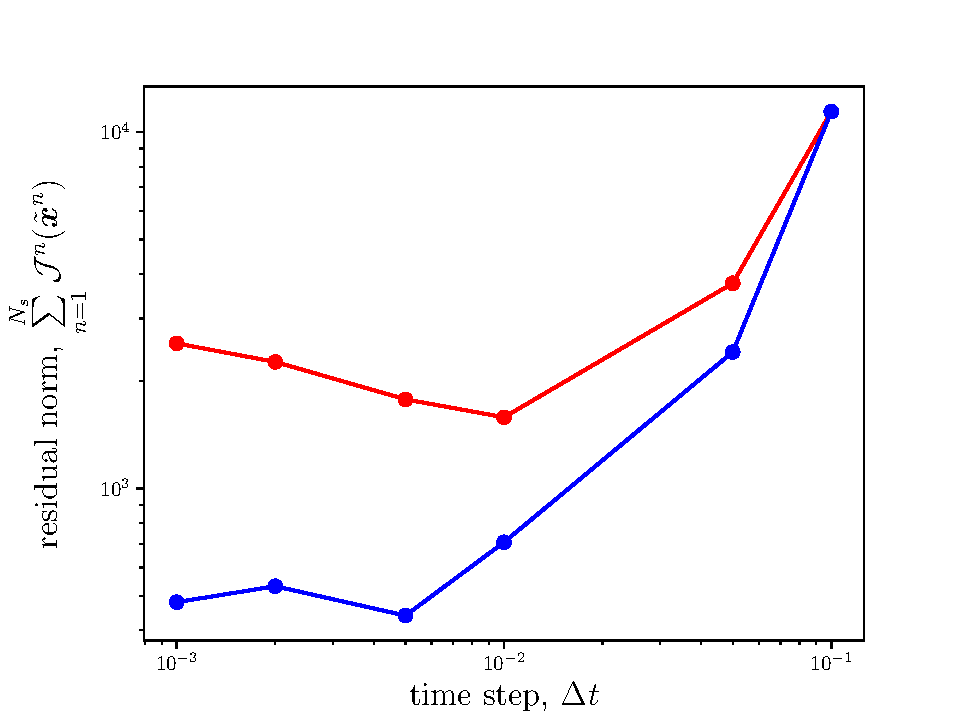
\includegraphics[width=1.\linewidth]{figs/sod/objective_vs_window_dtvar.pdf}
\caption{Space--time residual norm of the \methodAcronymROM.} 
\label{fig:sod_error_methods_b}
\end{subfigure}
\caption{Performance metrics of the Galerkin, LSPG, and \methodAcronymROMs.} 
\label{fig:time_step_study}
\end{center}
\end{figure}

\begin{figure}
\begin{center}
\begin{subfigure}[t]{0.45\textwidth}
%\includegraphics[width=1.\linewidth]{/Users/ejparis/PyROM/pyrom/sod/postProcess_wv/error_vs_window.pdf}
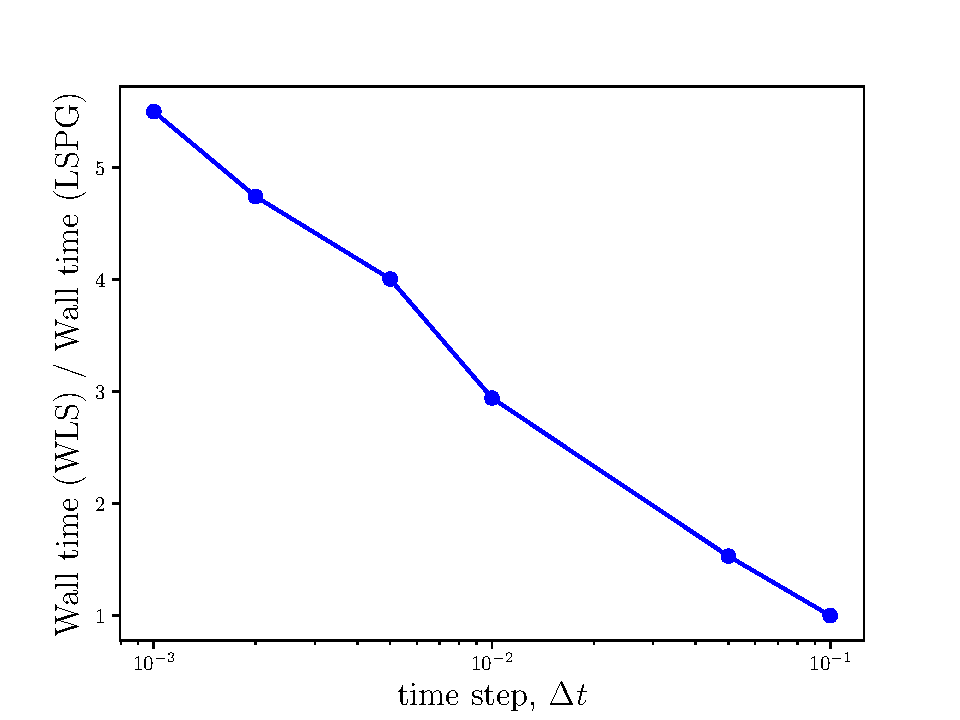
\includegraphics[width=1.\linewidth]{figs/sod/walltime_vs_window_dtvar.pdf}
\label{fig:sod_error_a}
\end{subfigure}
\caption{Comparison of wall-clock times of the \methodAcronymROMs\ to LSPG ROMs as a function of the time step. WLS ROMs have a fixed window size of $\Delta T = 0.1$.} 
\label{fig:walltime_dtvar}
\end{center}
\end{figure}


\subsubsection{Summary of numerical results for the Sod shock tube}
The key observations from the results of the first numerical example are: 
\begin{enumerate}
\item Increasing the window size over which the residual is minimized led to more physically relevant solutions. Specifically, we observed that as the window size over which the residual was minimized grew, \methodAcronym\ led to less oscillatory solutions.
\item Increasing the window size over which the residual is minimized does not necessary lead to a lower space--time state error as measured by the $\elltwo$ norm. We observed that minimizing the residual over an intermediary window size led to the lowest space--time state error in the $\elltwo$ norm. 
\item The \methodAcronym\ displays time-step convergence: both the space--time $\elltwo$ state error and residual norm decreased and displayed time-step convergence as the time step decreased. This is in contrast to LSPG.
\item For all examples considered, in where the windows comprised up to 2000 time instances, \methodAcronym\ with the direct method is between 1x and 10x the cost of the LSPG. The 
direct method was observed to be, in general, slightly more efficient and robust than the indirect method.
\end{enumerate} 

\subsection{Cavity Flow}
The next numerical example considers hyper-reduced ROMs of a viscous, compressible flow in a two-dimensional cavity. 
The flow is described by the two-dimensional compressible Navier-Stokes equations,
\begin{equation}\label{eq:compressible_ns}
\frac{\partial \mathbf{u}}{\partial t} + \nabla \cdot \big( \mathbf{F}(\mathbf{u} ) - \mathbf{F}_v (\mathbf{u},\nabla \mathbf{u} )      \big) =\bz,
\end{equation}
where $\mathbf{u}: [0,T] \times \Omega \rightarrow \RR{4}$ comprise the density, x and y momentum, and total energy. The terms $\mathbf{F}$ and $ \mathbf{F}_v$ are the inviscid and viscous fluxes, respectively. For a two-dimensional flow, the state vector and inviscid fluxes are
$$
\mathbf{u} = \begin{Bmatrix}
\rho \\ \rho u_1 \\ \rho u_2 \\ \rho E \end{Bmatrix}, \qquad \mathbf{F}_{1} = \begin{Bmatrix} \rho u_1 \\ \rho u_1^2 +      p \\ \rho u_1 u_2 \\ u_1(E + p) \end{Bmatrix}, 
\qquad \mathbf{F}_{2} = \begin{Bmatrix} \rho u_2 \\ \rho u_1 u_2  \\ \rho u_2^2 + p \\ u_2(E + p) \end{Bmatrix}.
$$
The viscous fluxes are given by
$$
\qquad \mathbf{F}_{v_1} = \begin{Bmatrix} 0 \\ \tau_{11} \\ \tau_{12}  \\ u_j \tau_{j1} + c_p \frac{\mu}{\text{Pr}} \frac{\partial T}{\partial x_1}  \end{Bmatrix}, 
\qquad \mathbf{F}_{v_2} = \begin{Bmatrix} 0 \\ \tau_{21} \\ \tau_{22}  \\ u_j \tau_{j2} + c_p \frac{\mu}{\text{Pr}} \frac{\partial T}{\partial x_2}  \end{Bmatrix}.
$$
We assume a Newtonian fluid, which leads to a viscous stress tensor of the form,
\begin{equation*}
\tau_{ij} = 2\mu S_{ij},
\end{equation*}
where,
\begin{equation*}
 S_{ij} = \frac{1}{2} \big( \frac{\partial u_i}{\partial \mathsf{x}_j} + \frac{\partial u_j}{\partial \mathsf{x}_i} \big) - \frac{1}{3} \frac{\partial      u_k}{\partial \mathsf{x}_i} \delta_{ij}.
\end{equation*}
The Navier-Stokes equations are closed with a constitutive relationship for a calorically perfect gas,
$$p = (\gamma - 1)( \rho E - \frac{1}{2} \rho u_1^2 - \frac{1}{2} \rho u_2^2 \big),$$
where $\gamma = 1.4$ is the heat-capacity ratio.

Figure~\ref{fig:cav_fig} depicts the domain $\Omega$ and flow conditions. Free-stream boundary conditions 
are used at the inlet, outlet, and top wall of the cavity. No-slip boundary conditions are enforced 
on the bottom wall of the cavity. 

\subsubsection{Description of FOM and Generation of Trial Space}
The full-order model comprises a discontinuous-Galerkin discretization. The discretization 
is obtained by partitioning the domain into $100$ elements in the flow direction and $40$ elements 
in the wall-normal direction. The solution is represented to third order over each element using tensor product polynomials of order $p=2$, 
resulting in $36000$ unknowns for each conserved variable. Spatial discretization via the discontinuous Galerkin method yields a dynamical system 
of the form,
$$\frac{d \state}{dt} = \mass_{\text{DG}} \velocity_{\text{DG}} (\state),$$
where $\mass_{\text{DG}} \in \RR{N \times N}$ is the DG mass matrix and $\velocity_{\text{DG}}: \RR{N} \rightarrow \RR{N}$ is the DG velocity operator containing 
surface and volume integrals. By the definition of the FOM~\eqref{eq:FOM}, the dynamical system velocity is $\velocity = \mass_{\text{DG}} \velocity_{\text{DG}}$. 
Figure~\ref{fig:cav_mesh} shows the computational mesh. The 
DG method leverages the Rusanov flux at the cell interfaces~\cite{rusanov} and uses the first form of Bassi and Rebay~\cite{br1} for the viscous fluxes. Time integration 
is performed via a third-order strong stability preserving Runge-Kutta method~\cite{ssp_rk3} with a time-step size of $\Delta t = 0.001$. 
 
The reduced-order models leverage POD to construct the trial basis and use q-sampling~\cite{qdeim_drmac} based on snapshots of the FOM velocity to construct the weighting 
matrix $\stweightingMatArg{n}$. The process used to construct the initial conditions and trial spaces for the ROMs are as follows:
\begin{enumerate}
\item Initialize the FOM with uniform free-stream conditions.
\item Evolve the FOM for $t \in [0,400]$.
\item Reset the time-coordinate, $0 \leftarrow t$, and execute Algorithm~\ref{alg:pod} with $\stateInterceptArg{} = \bz, N_{\text{skip}} = 100$ and $K = \{136,193\}$ over $t \in [0,100]$ to construct two trial spaces comprising $\approx 95\%$ and $\approx 97\%$ of the snapshot energy, respectively. 
\item Execute Algorithm~\ref{alg:qdeim} with $N_{\text{skip}} = 100$, $n_s = 129$ to obtain the sampling point matrix of dimension $\stweightingMatOneArg{} \in \{0,1\}^{1603 \times \fomdim }$. 
\end{enumerate}
Figure~\ref{fig:cav_sampmesh} shows the resulting sample mesh used in the ROM simulations. To depict the nature of the flow, Figure~\ref{fig:fom_sols_cav} shows snapshots of the vorticity field generated by the FOM for several time instances used in training.  
\begin{table}[]
\begin{centering}
\begin{tabular}{c c c c}
\hline
Basis \# & Trial Basis Dimension ($K$) &  Energy Criterion & Sample Points ($n_S$) \\
\hline
%1    & $136$ & $95.0\%$ & $580$ \\
%2    & $193$ & $97.0\%$ & $580$ \\
1    & $136$ & $95.0\%$ & $1603$ \\
2    & $193$ & $97.0\%$ & $1603$ \\
\hline
\end{tabular}
\caption{Summary of the various basis sizes employed in the cavity flow example.}
\label{tab:rom_basis_details}
\end{centering}
\end{table}

\subsubsection{Description of Reduced-Order Models}
Hyper-reduced ROMs based on the Galerkin, collocated Least--Squares Petrov--Galerkin, and \methodAcronym\ approaches are 
again considered. Details on the implementation of the methods is as follows:
\begin{itemize}
\item \textbf{Galerkin ROM with Collocation}: The Galerkin ROM with collocation is obtained through Galerkin projection of the FOM. Unless 
otherwise noted, the  Galerkin ROM is evolved in time with the Crank--Nicolson time scheme at a time step of $\Delta t =0.1$.

\item \textbf{LSPG ROM with Collocation}: The LSPG ROM with collocation is built on top of the FOM discretization using the Crank--Nicolson scheme for temporal 
discretization. Unless otherwise noted, the time step for the LSPG ROM is $\Delta t  = 0.1$. As in the previous example, 
the Gauss--Newton method is used to solve the non-linear least-squares problem arising at each time instance. The Gauss--Newton 
algorithm is deemed converged when the gradient norm is less than $1e-4$. All Jacobians are again computed via automatic differentiation.
 
\item \textbf{\methodAcronymROMs\ with Collocation}: \methodAcronymROMs\ are solved via the direct method. The ROMs use the Crank--Nicolson time-discretization with a time-step size of 
$\Delta t = 0.1$. The Gauss--Newton algorithm is deemed converged when the gradient norm is less than $1e-4$. All Jacobians are computed via automatic differentiation. Uniform quadrature 
weights are used for evaluating the integral in~\eqref{eq:obj_gen_slab}. 
 
%\begin{itemize}
%\item Direct Method: \methodAcronym ROMs solved via the direct method are again implemented with the same Crank--Nicolson time discretization with a nominal 
%time-step size of $\Delta t = 0.1$. 
%\end{itemize}
\end{itemize}


\begin{figure}
\begin{center}
%\begin{subfigure}[t]{0.85\textwidth}
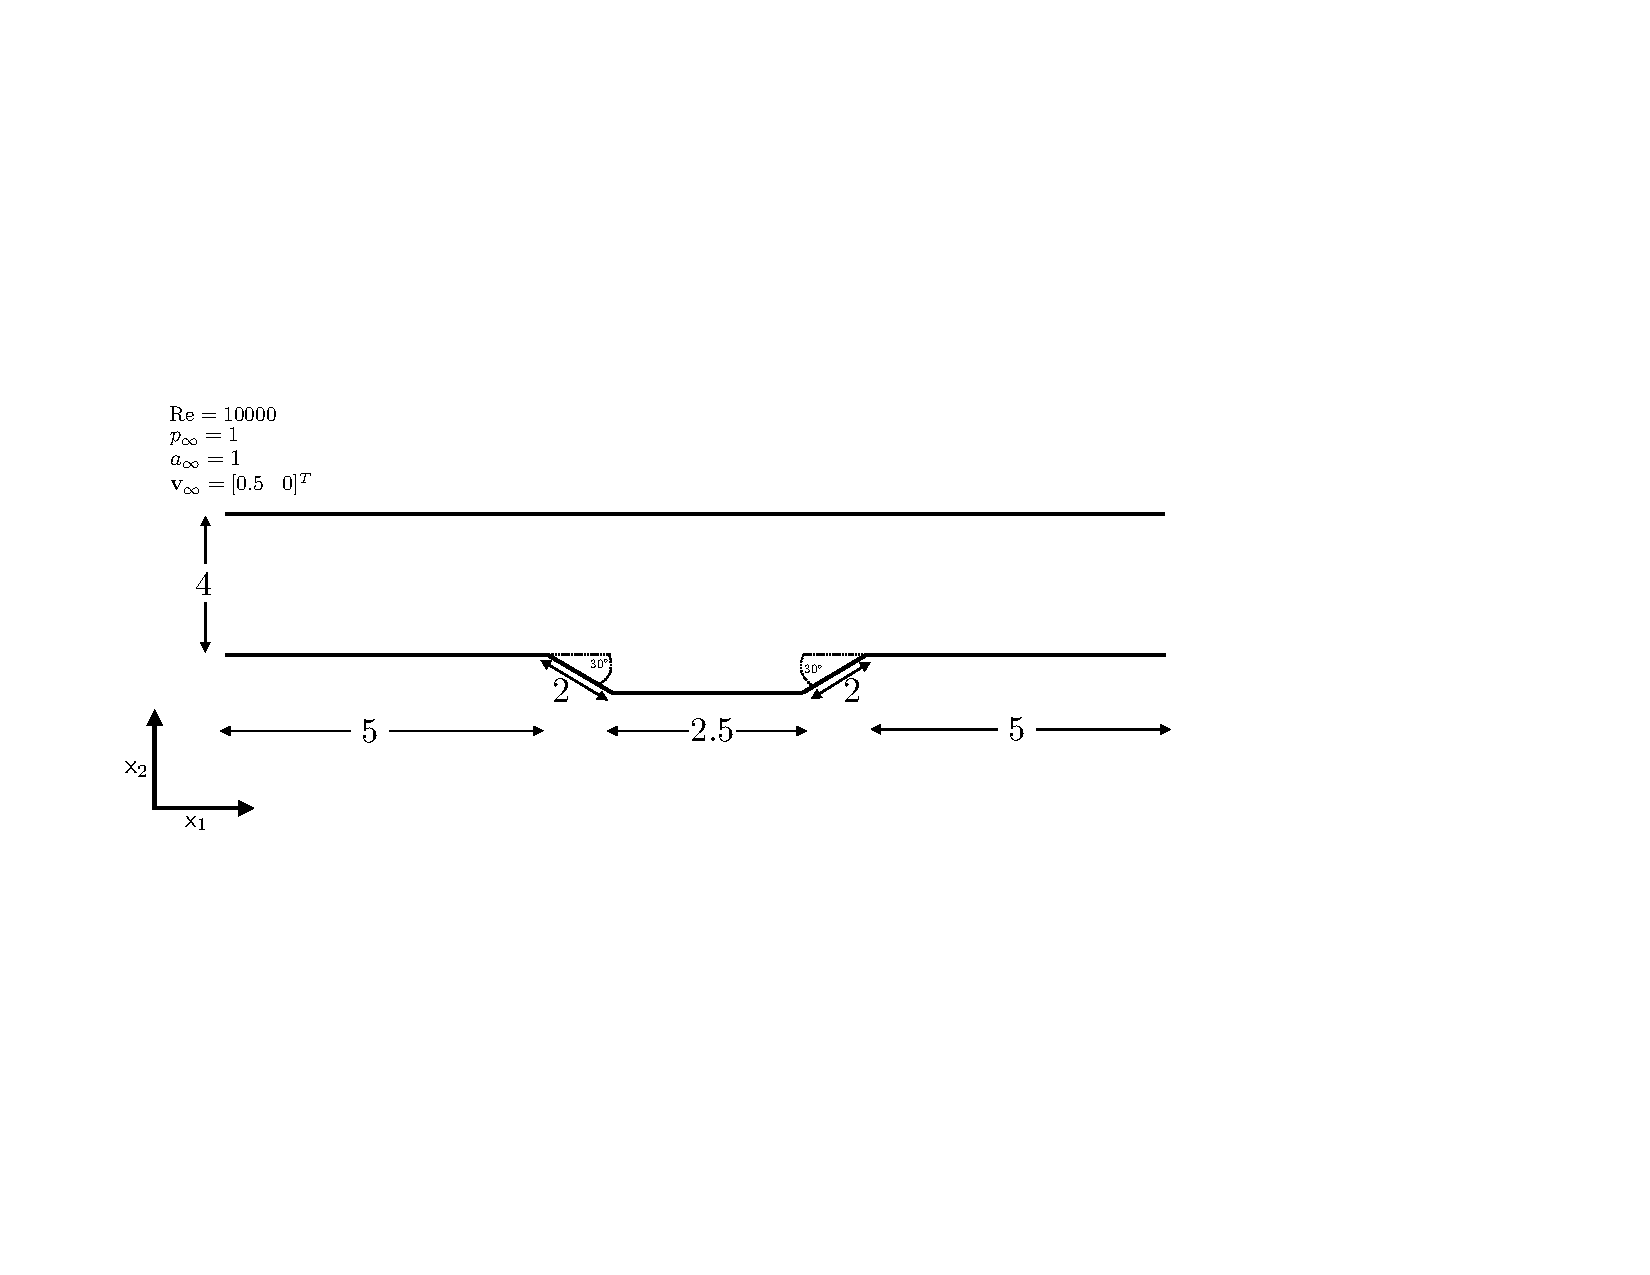
\includegraphics[trim={2cm 7cm 4cm 6cm},clip,width=0.95\linewidth]{cav_fig.pdf}
%\end{subfigure}
\caption{Figure depicting geometry and flow conditions of the cavity flow problem.} 
\label{fig:cav_fig}
\end{center}
\end{figure}

\begin{figure}
\begin{center}
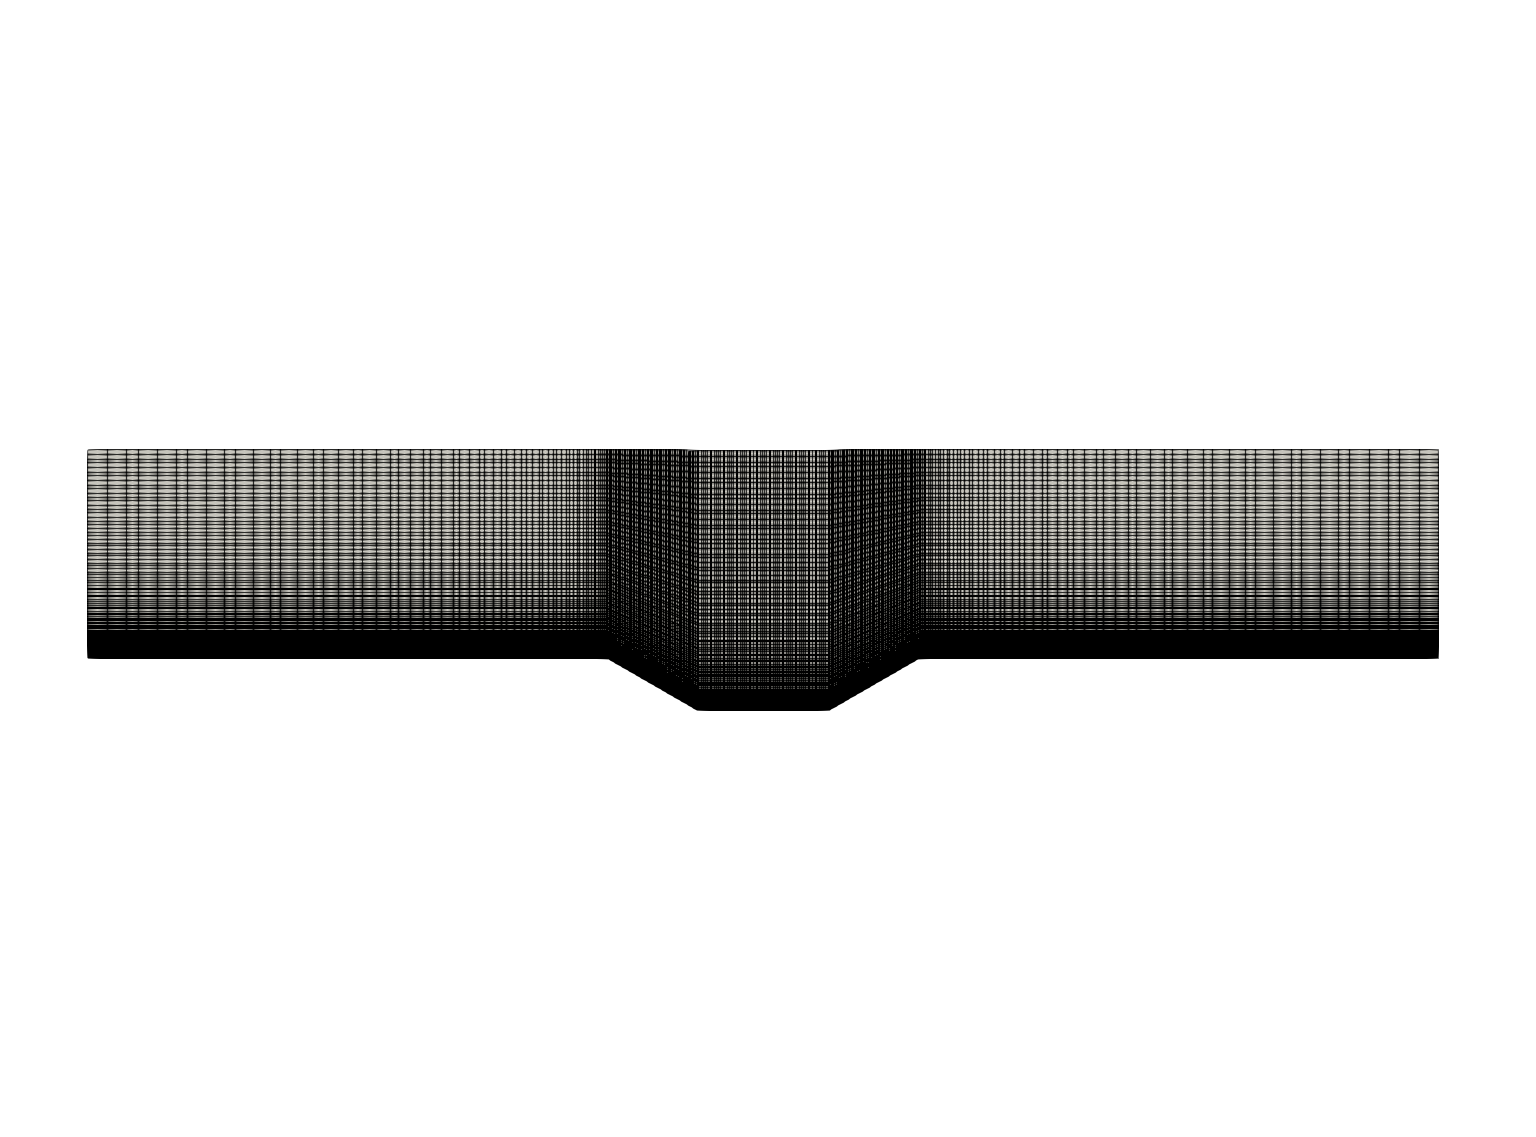
\includegraphics[trim={0cm 14cm 0cm 14cm},clip,width=1.\linewidth]{figs/cavity/grid.png}
\caption{Computational mesh}
\label{fig:cav_mesh}
\end{center}
\end{figure}

\begin{figure} 
\begin{center}
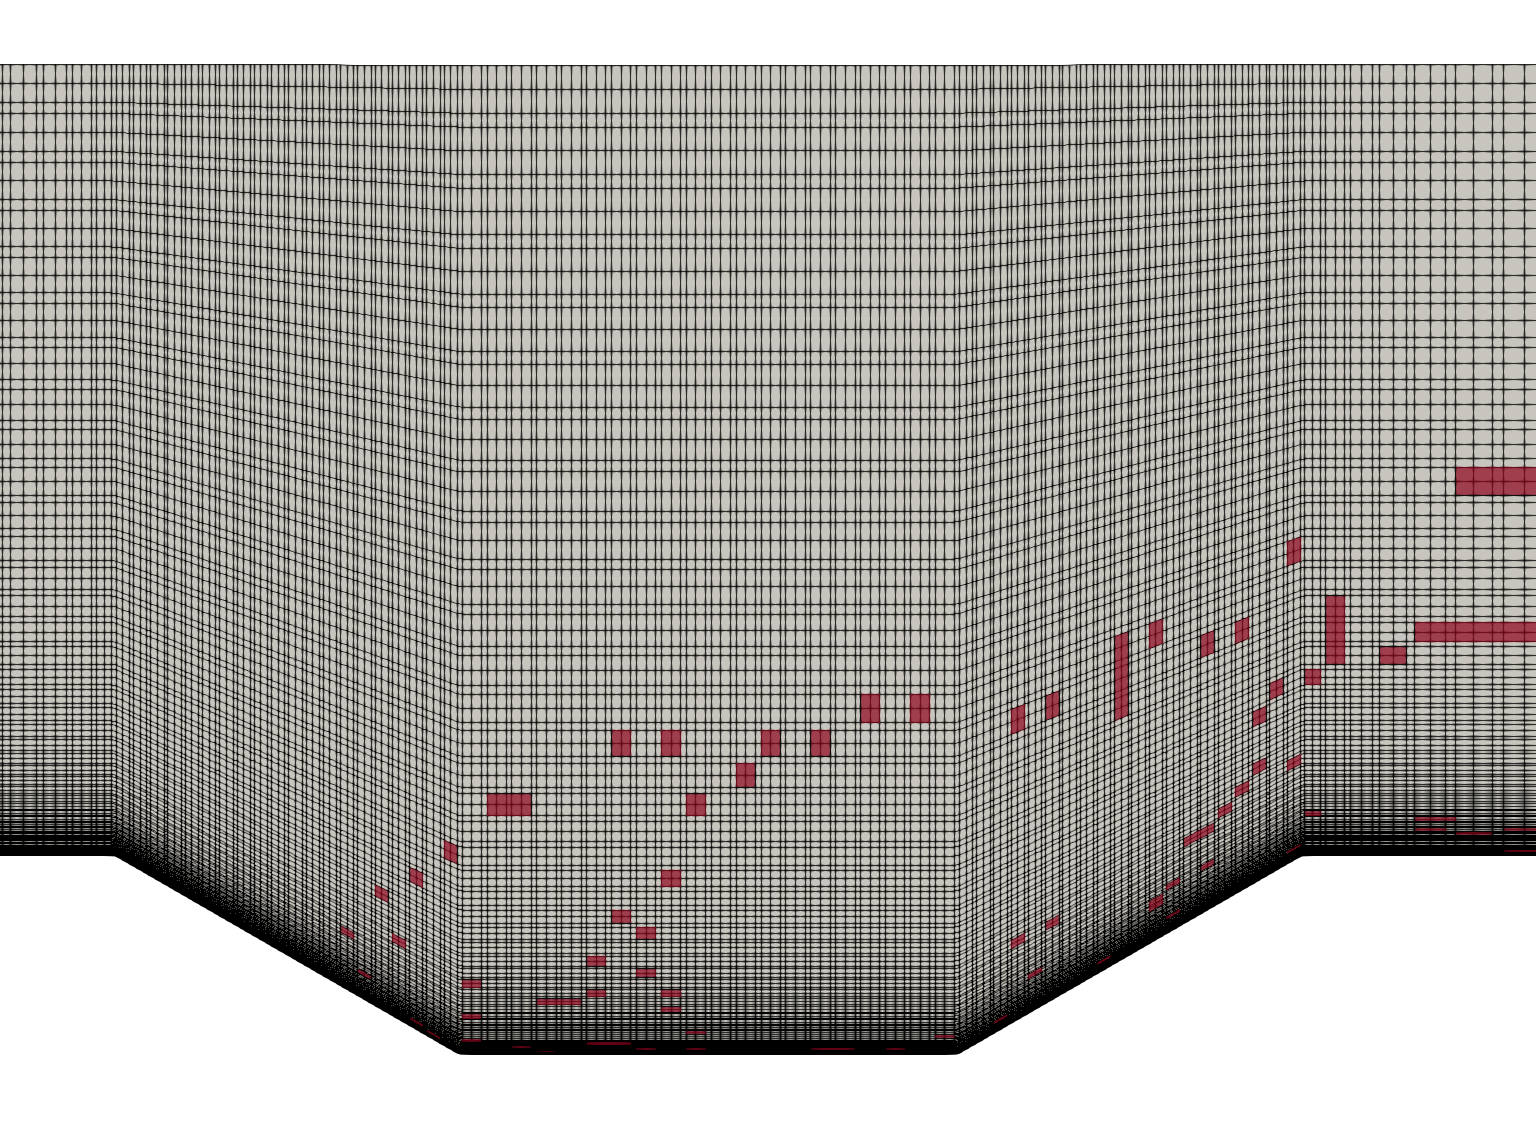
\includegraphics[trim={0cm 0cm 0cm 0cm},clip,width=0.65\linewidth]{figs/cavity/hyper_grid.png}
\caption{Close up of computational mesh with highlighted collocation cells} 
\label{fig:cav_sampmesh}
\end{center}
\end{figure}

\begin{figure}
\begin{center}
%\begin{subfigure}[t]{0.85\textwidth}
\begin{subfigure}[t]{0.49\textwidth}
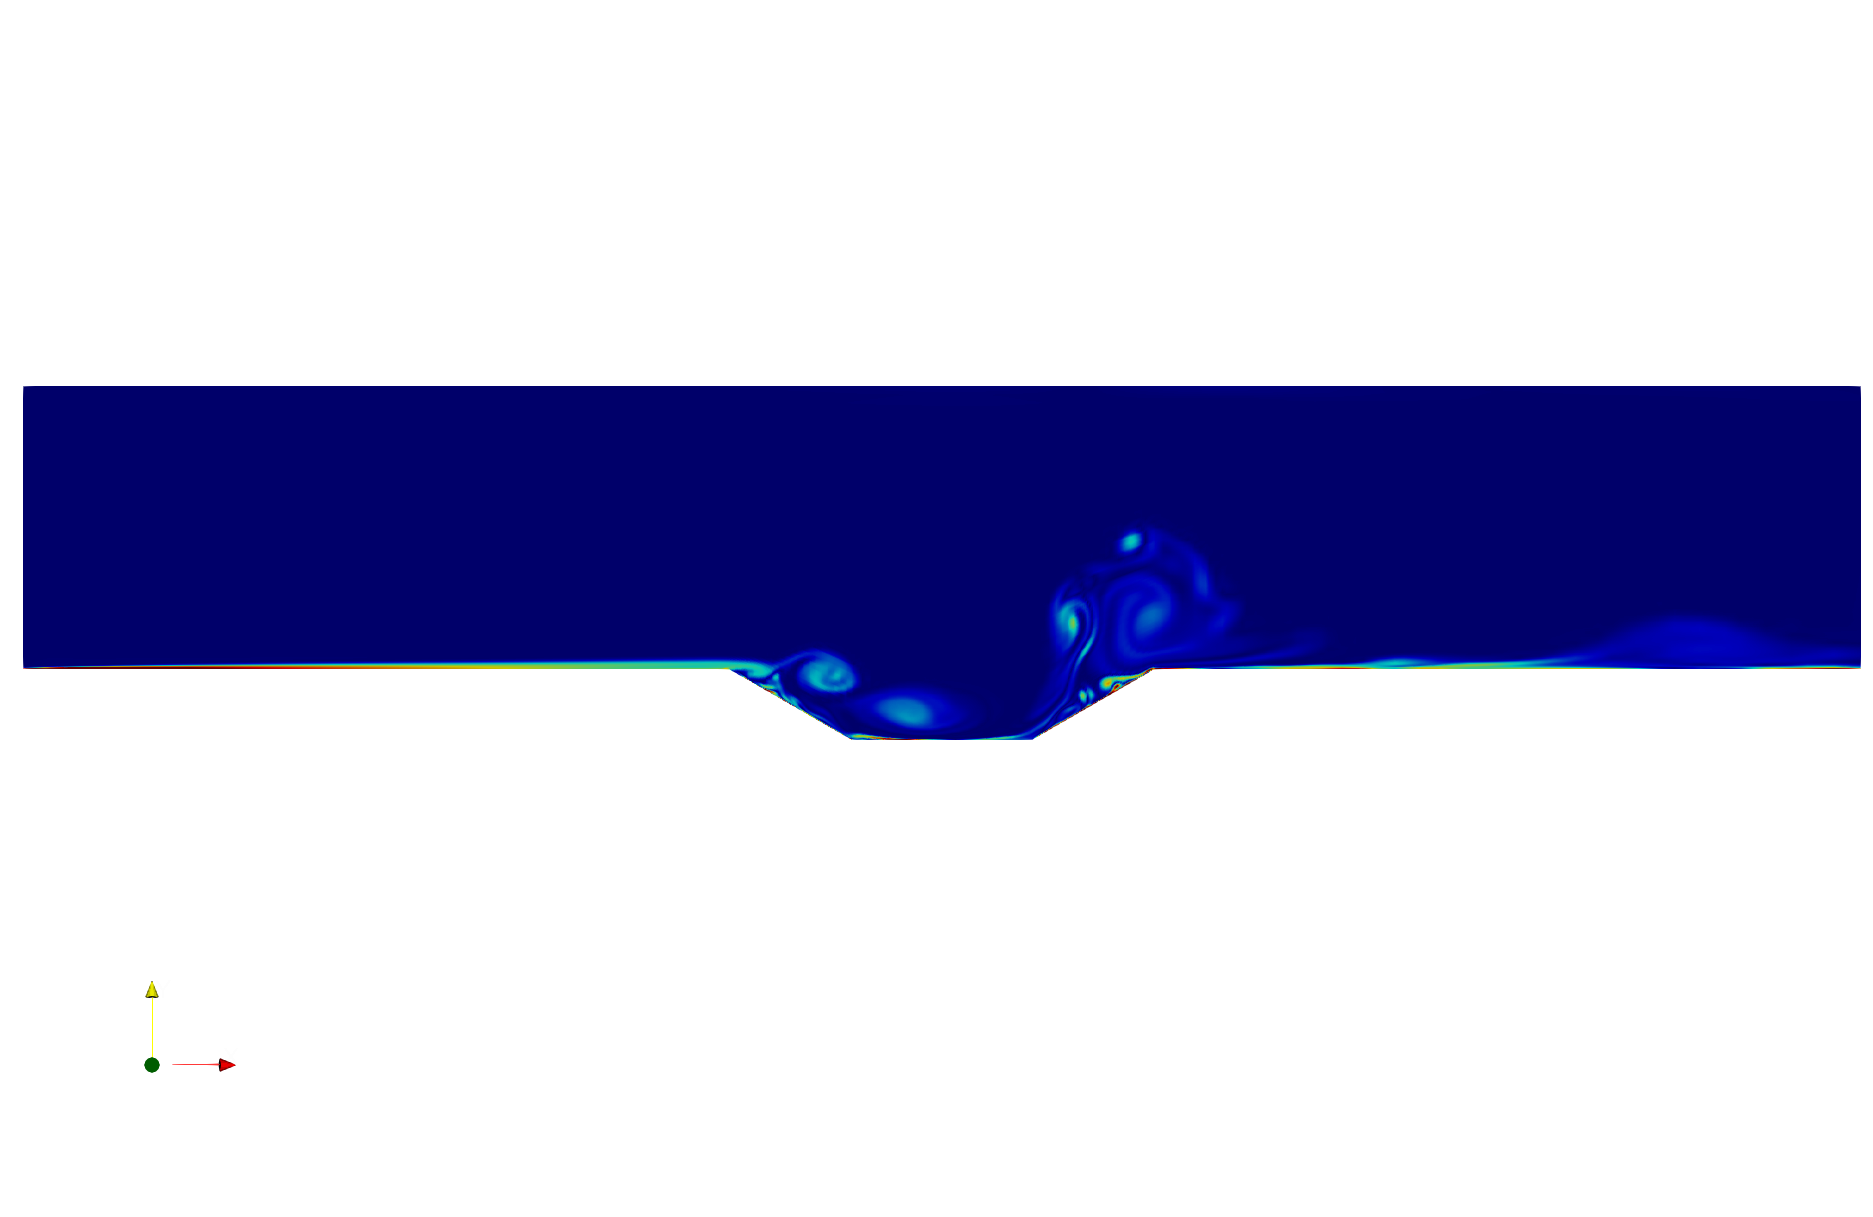
\includegraphics[trim={18cm 16cm 18cm 15cm},clip,width=1.0\linewidth]{figs/cavity/animate/sol0000.png}
\caption{$t=0.0$}
\end{subfigure}
\begin{subfigure}[t]{0.49\textwidth}
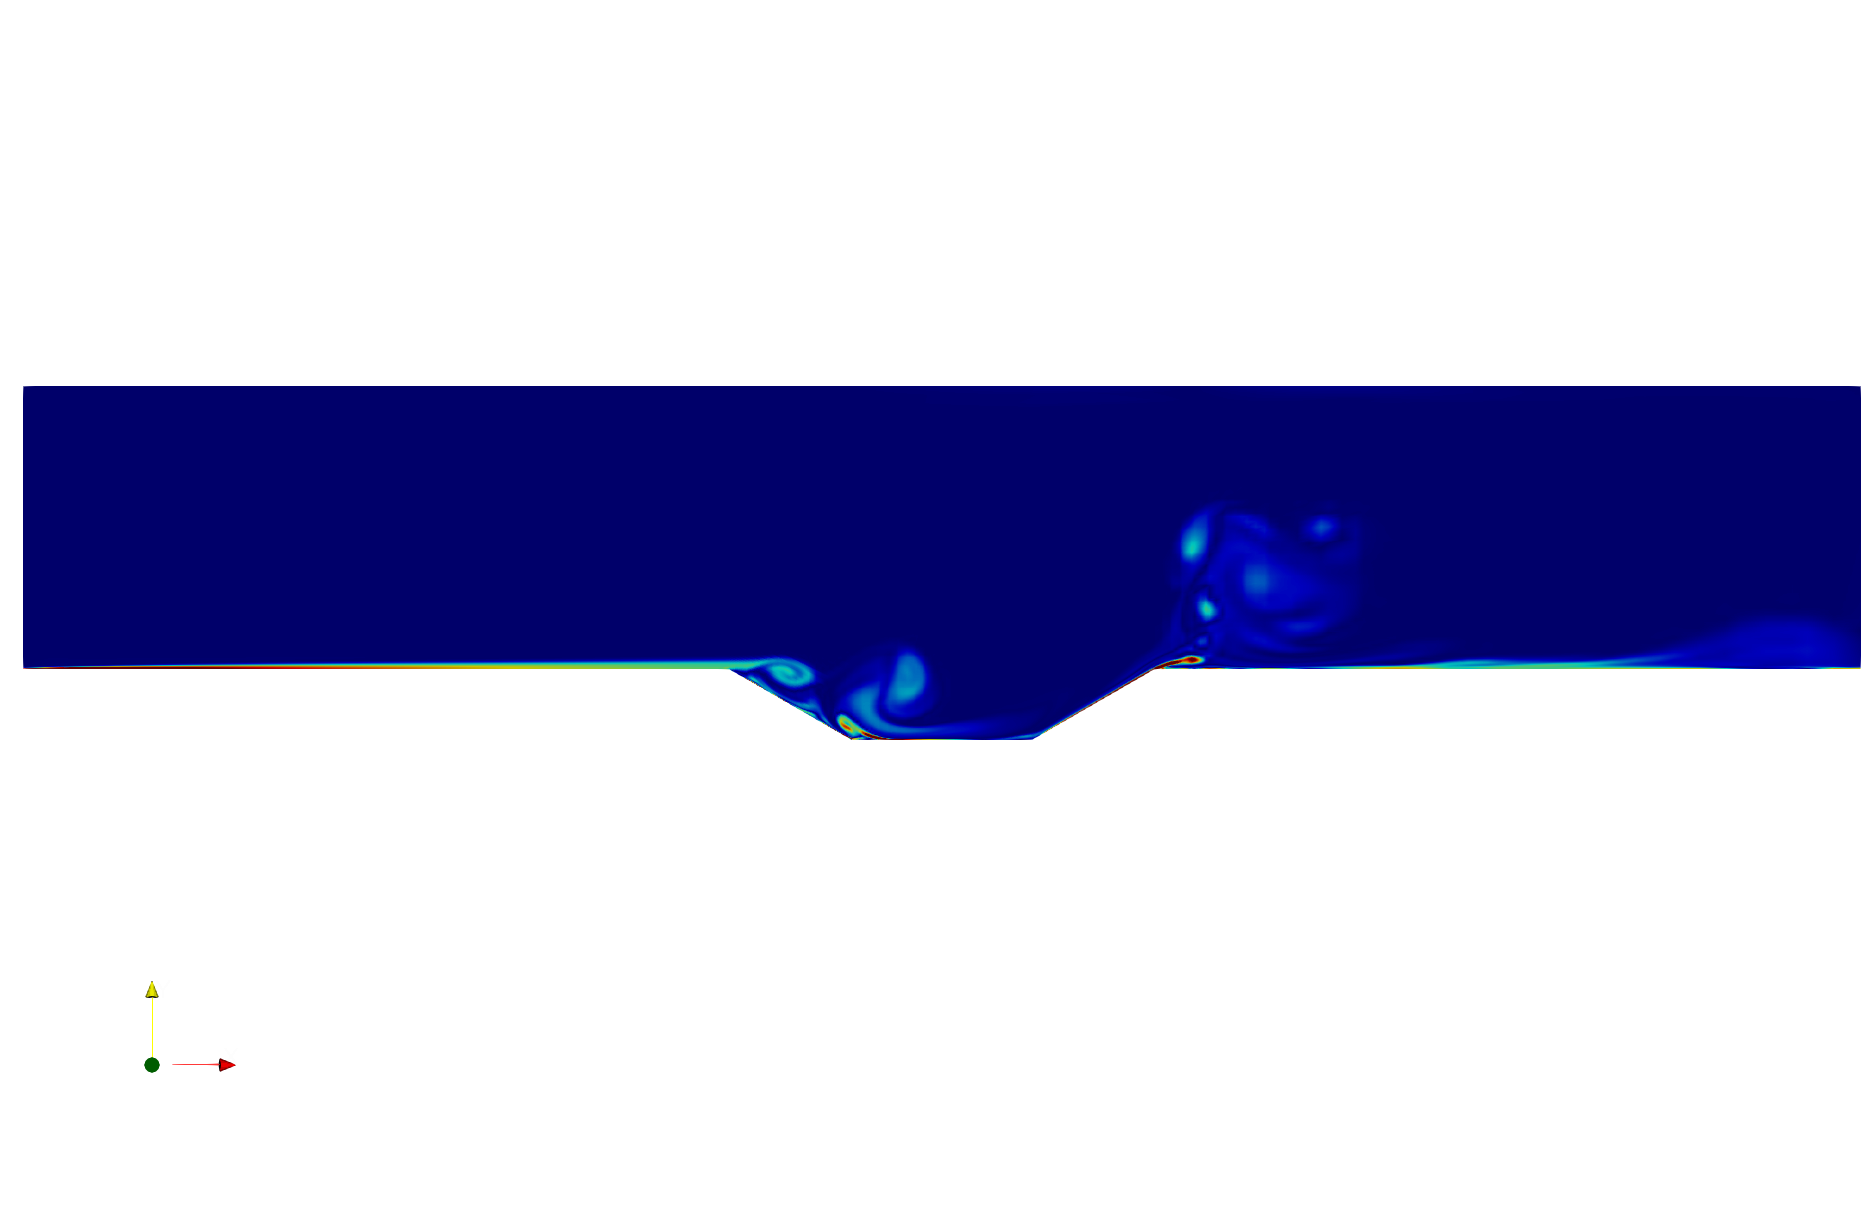
\includegraphics[trim={18cm 16cm 18cm 15cm},clip,width=1.0\linewidth]{figs/cavity/animate/sol0040.png}
\caption{$t=4.0$}
\end{subfigure}
\begin{subfigure}[t]{0.49\textwidth}
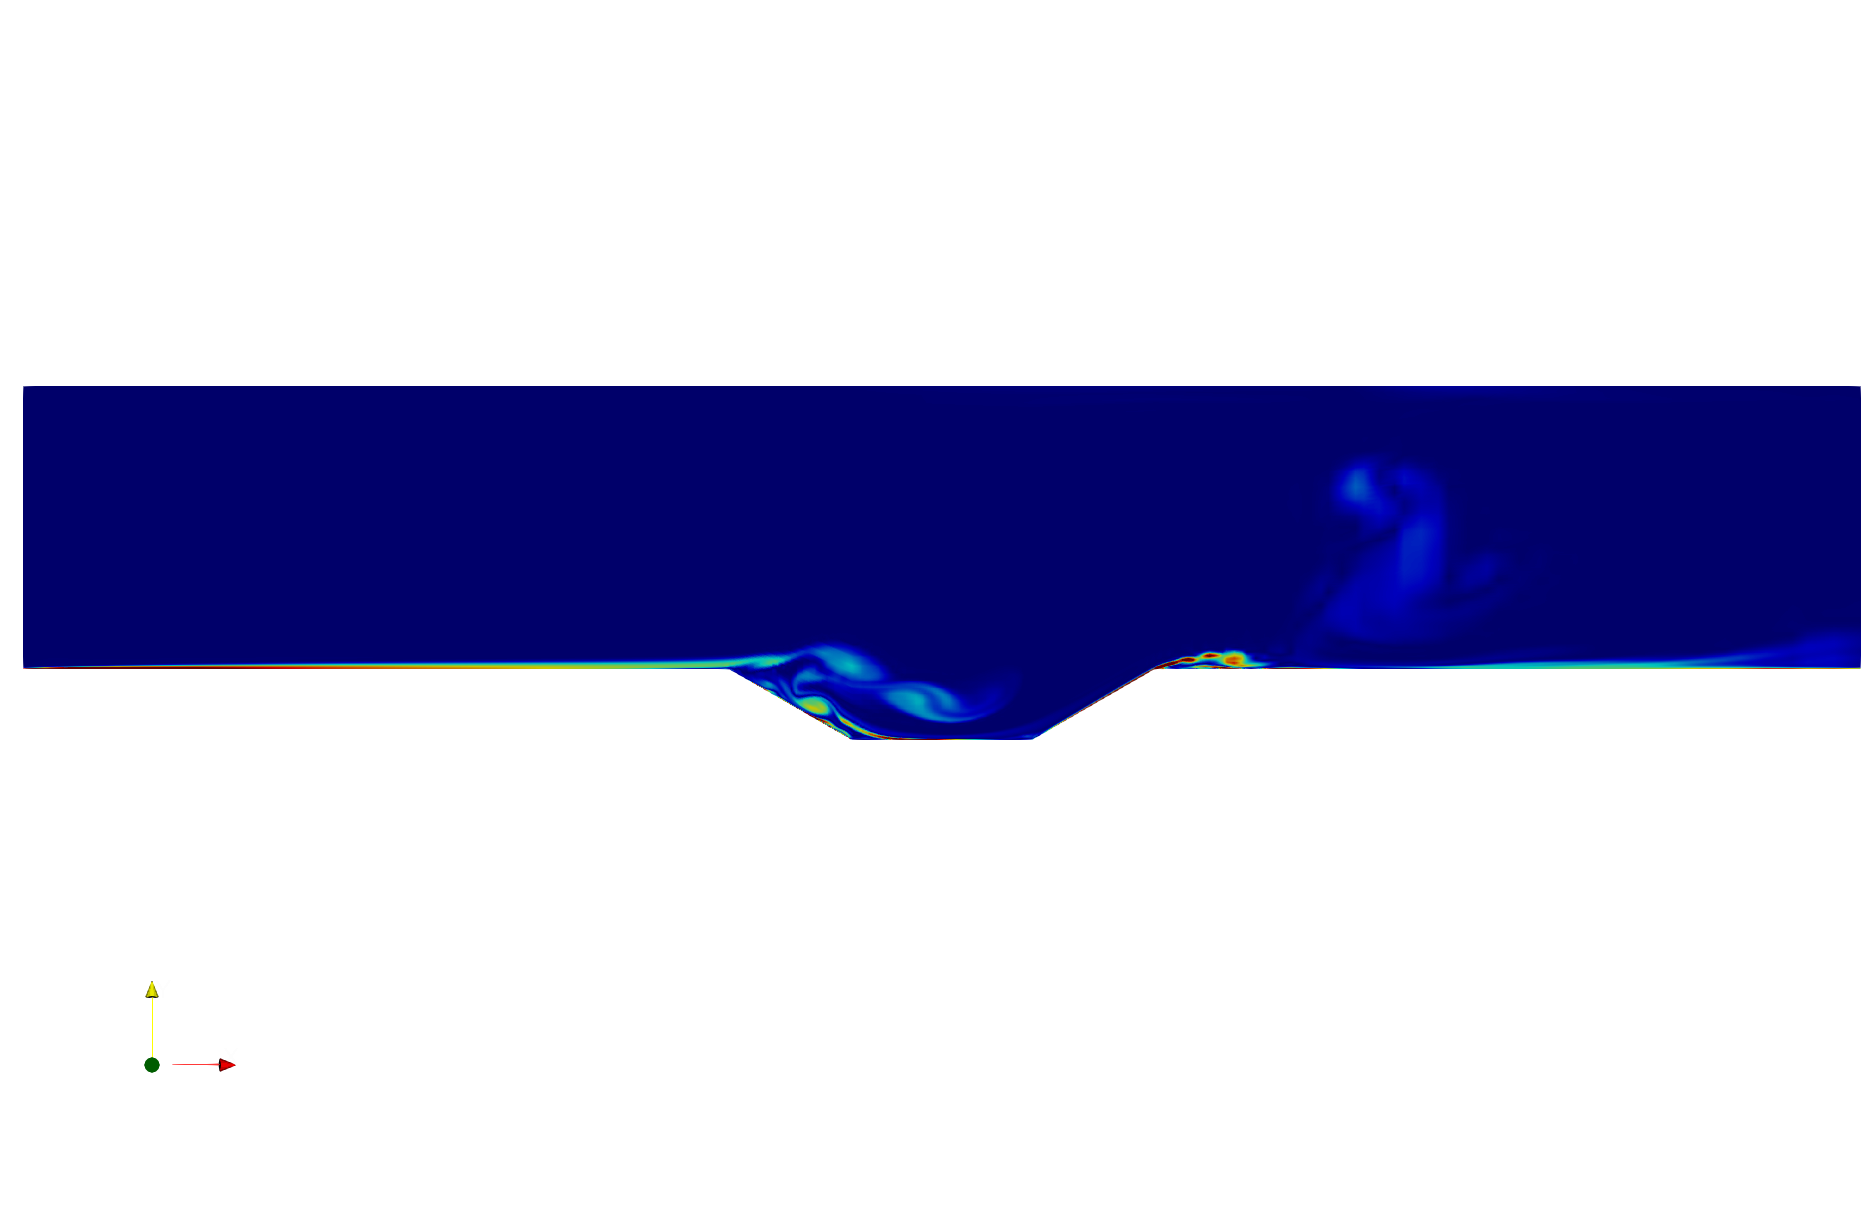
\includegraphics[trim={18cm 16cm 18cm 15cm},clip,width=1.0\linewidth]{figs/cavity/animate/sol0080.png}
\caption{$t=8.0$}
\end{subfigure}
\begin{subfigure}[t]{0.49\textwidth}
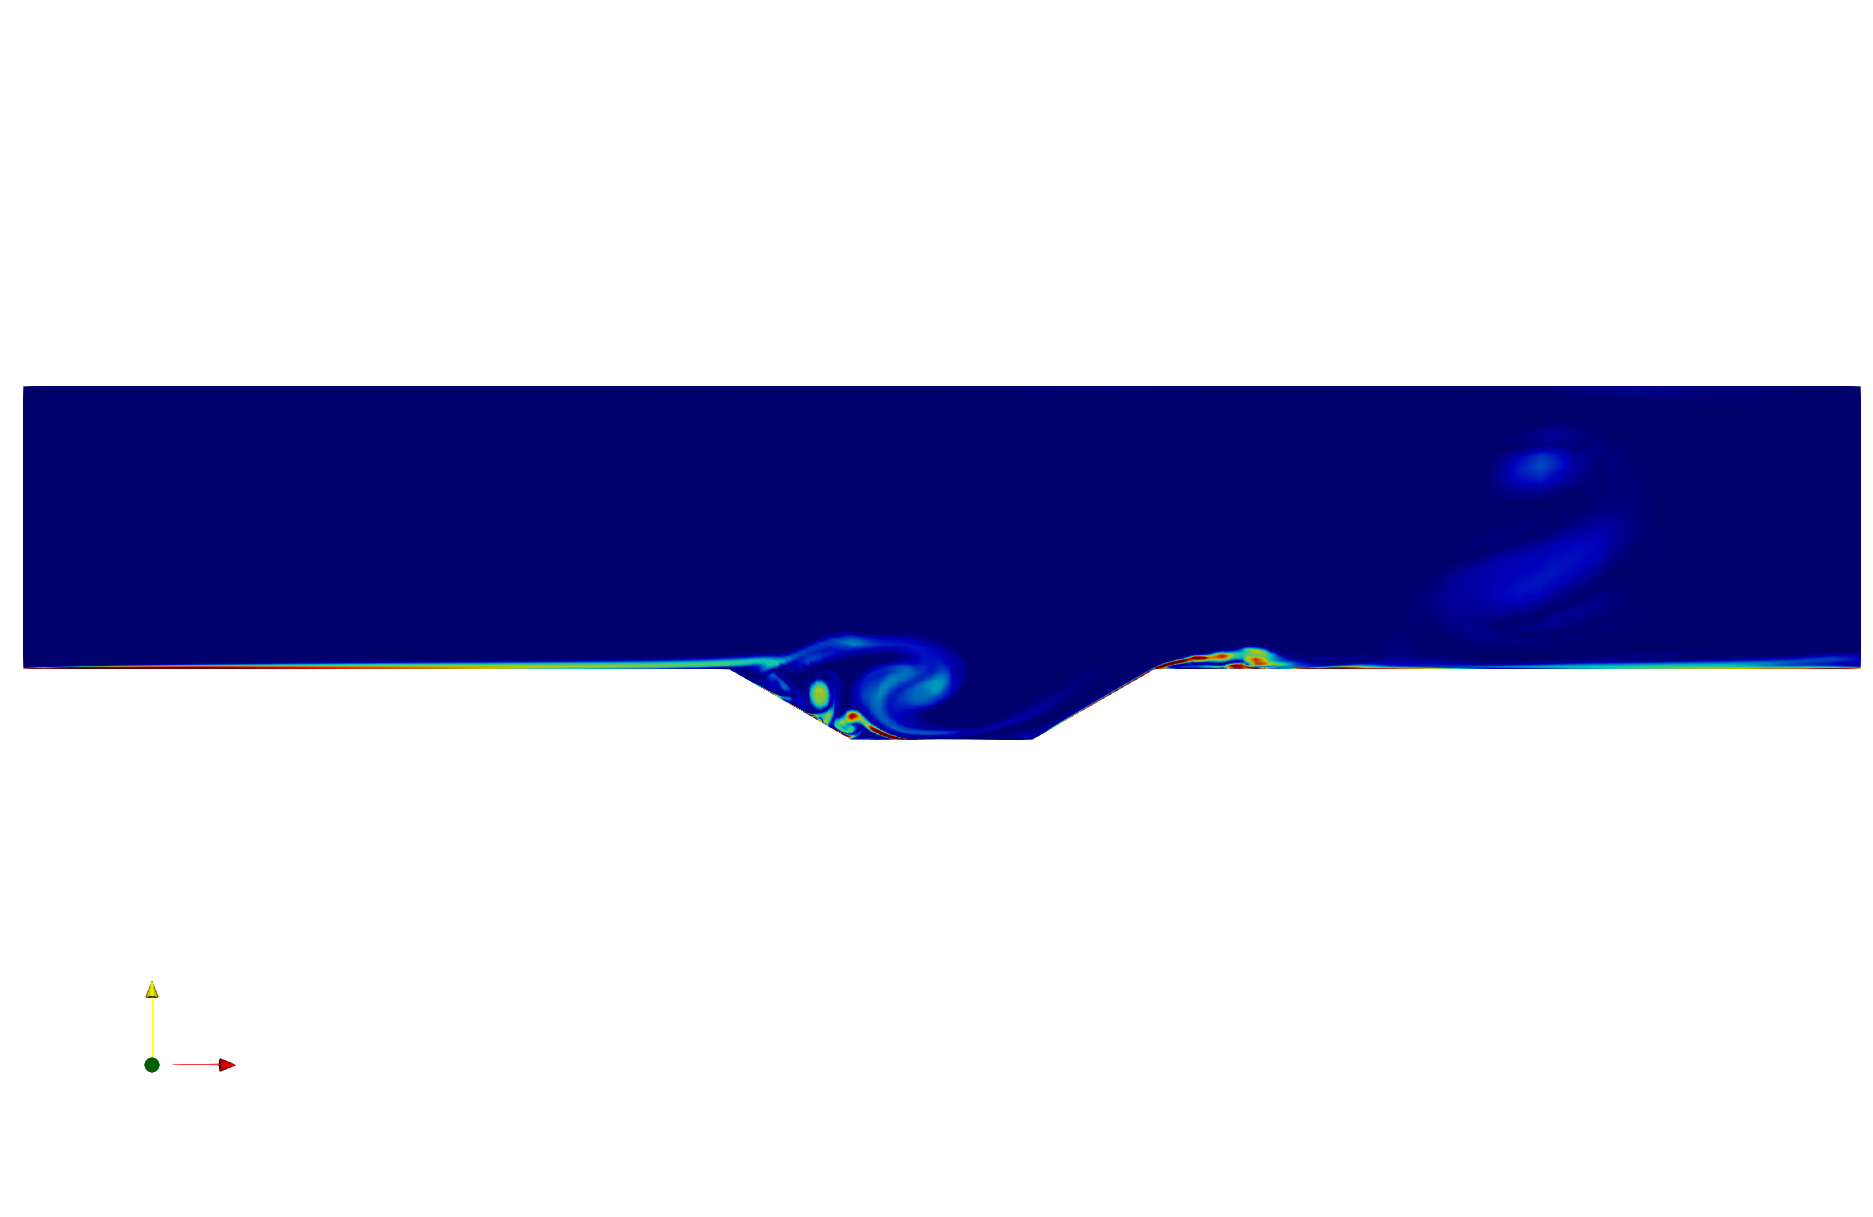
\includegraphics[trim={18cm 16cm 18cm 15cm},clip,width=1.0\linewidth]{figs/cavity/animate/sol0120.png}
\caption{$t=12.0$}
\end{subfigure}
\begin{subfigure}[t]{0.49\textwidth}
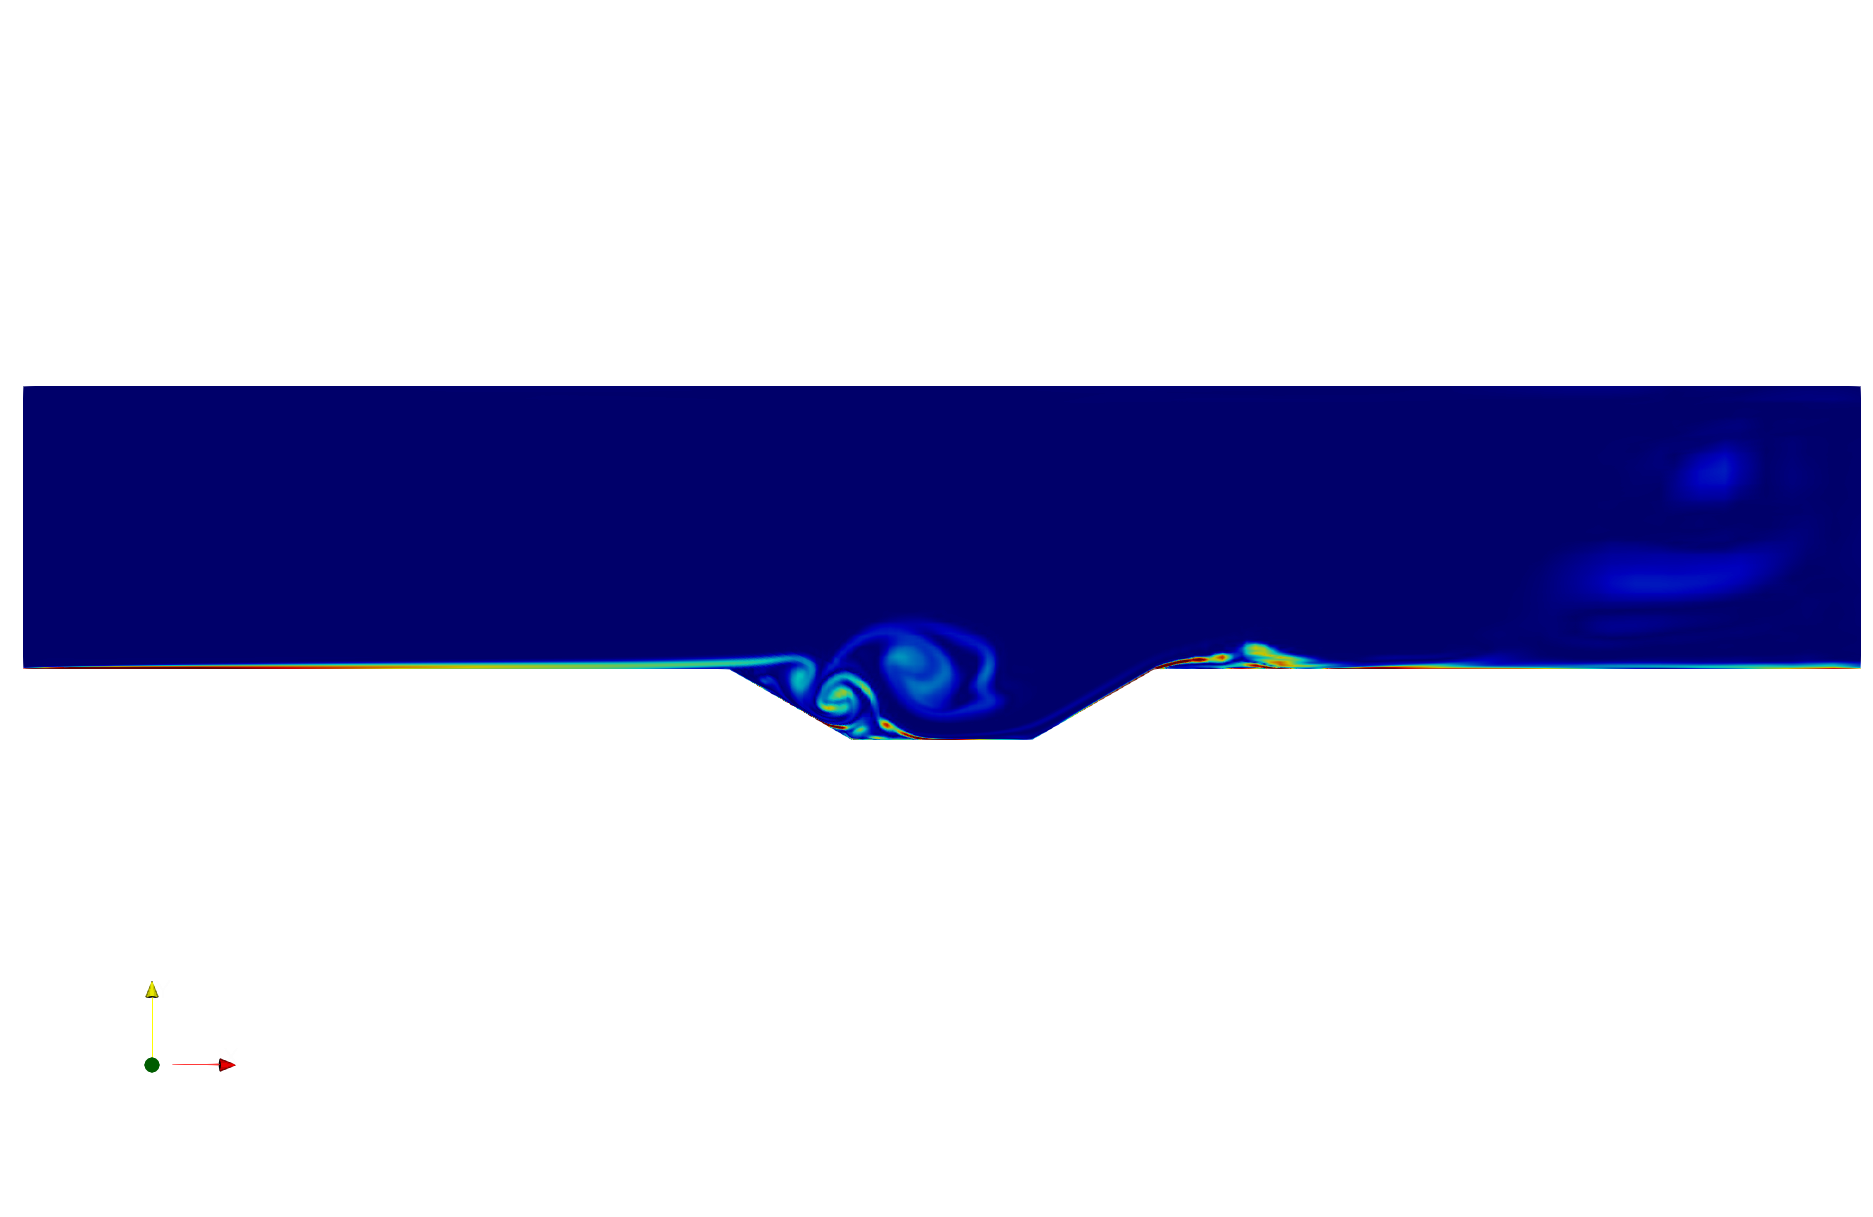
\includegraphics[trim={18cm 16cm 18cm 15cm},clip,width=1.0\linewidth]{figs/cavity/animate/sol0160.png}
\caption{$t=16.0$}
\end{subfigure}
\begin{subfigure}[t]{0.49\textwidth}
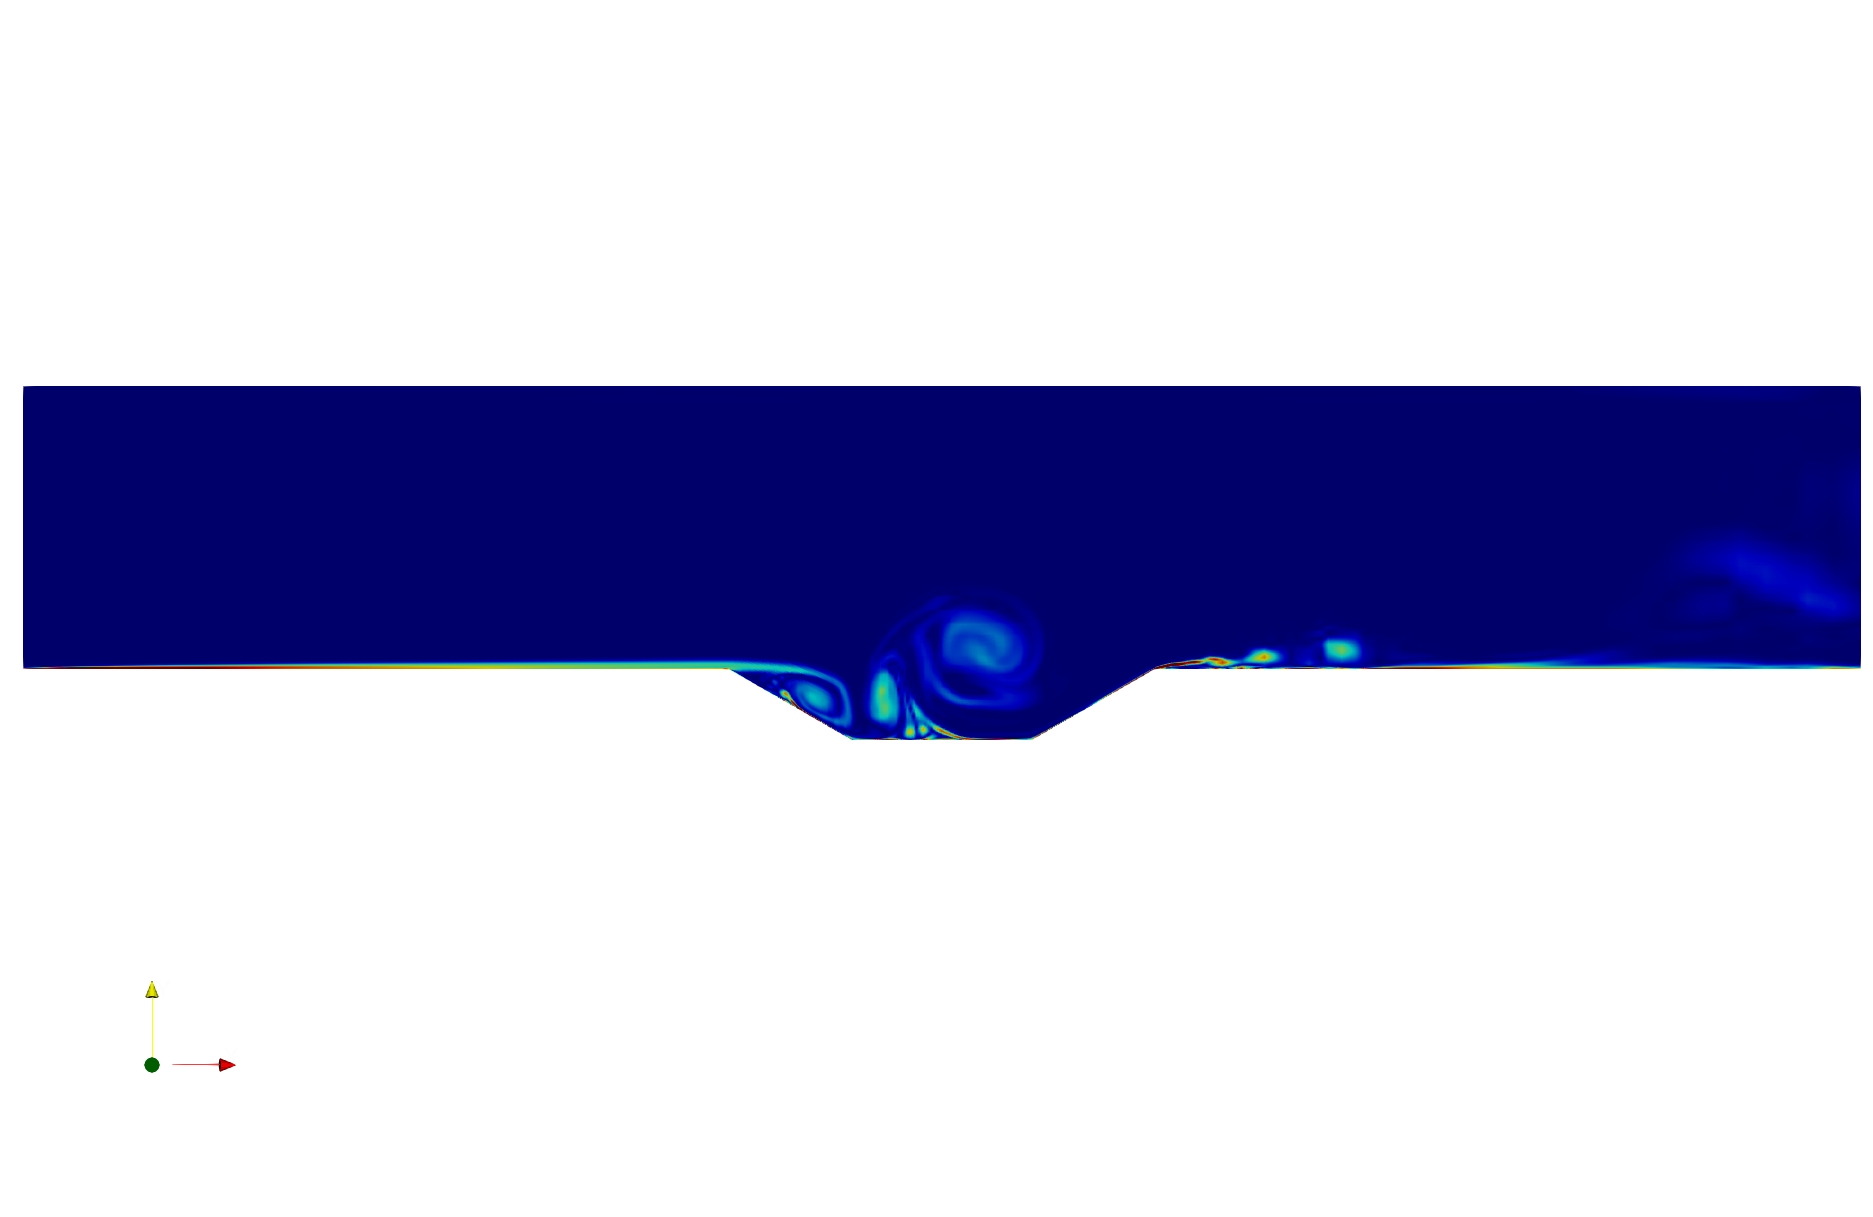
\includegraphics[trim={18cm 16cm 18cm 15cm},clip,width=1.0\linewidth]{figs/cavity/animate/sol0200.png}
\caption{$t=20.0$}
\end{subfigure}
\caption{Vorticity snapshots from the FOM simulation at various time instances.} 
\label{fig:fom_sols_cav}
\end{center}
\end{figure}


\subsubsection{Numerical Results}
We first assess the performance of \methodAcronymROMs\ with varying window sizes. To this end, we consider \methodAcronymROMs\ with uniform window 
sizes of $\Delta T^n \equiv \Delta T = 0.2,0.5,1.0,$ and $2.0$, along with the Galerkin and LSPG ROMs. Results are first considered for basis \#1 as described in 
Table~\ref{tab:rom_basis_details}. For all ROMs, we evolve 
the solution for $t \in [0,100]$. This comprises the same time interval used to construct the trial space. First, Figure~\ref{fig:cav_results1a} depicts the evolution of the pressure at the bottom wall in the midpoint of the computational domain, while Figure~\ref{fig:cav_results1b} depicts the evolution of the normalized $\elltwo$ state error of the various reduced-order models. Both the hyper-reduced Galerkin and LSPG ROMs blow up/fail to converge within the first several time units. The \methodAcronymROM\ minimizing the residual over a window of size $\Delta T = 0.2$ also fails to converge. The \methodAcronymROMs\ that minimize the residual over window sizes of $\Delta T \ge 0.5$ are seen to all be stable and accurate; the pressure response is well characterized and the normalized state errors are again less than $10\%$. The most notable discrepancy between the \methodAcronymROM\ and FOM solutions is a slight phase difference. 






\begin{figure}
\begin{center}

\begin{subfigure}[t]{0.95\textwidth}
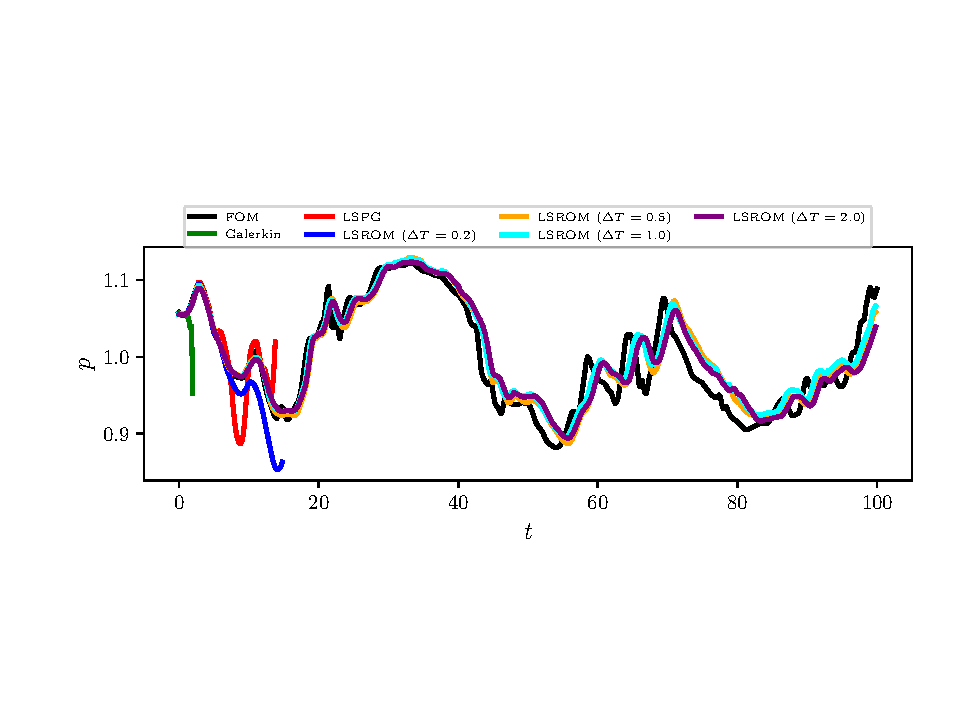
\includegraphics[trim={0cm 3.0cm 0cm 3cm},clip,width=1.\linewidth]{figs/cavity/pressure_basis2.pdf}
\caption{Pressure} 
\label{fig:cav_results1a}
\end{subfigure}

\begin{subfigure}[t]{0.95\textwidth}
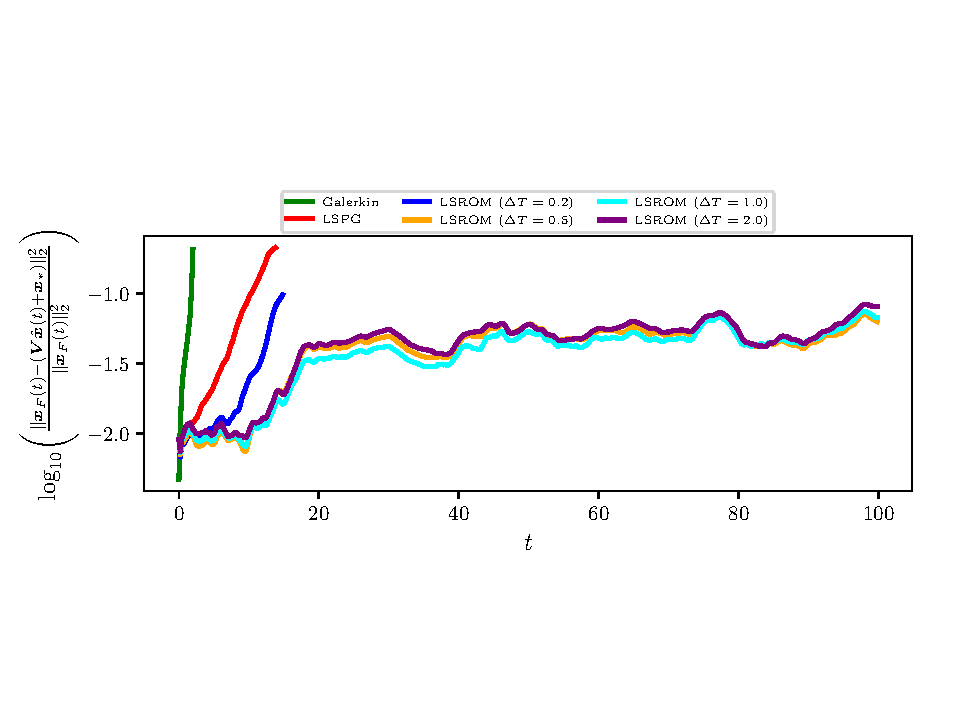
\includegraphics[trim={0cm 2.8cm 0cm 3cm},clip,width=1.\linewidth]{figs/cavity/error_basis2.pdf}
\caption{Normalized $\elltwo$ error}
\label{fig:cav_results1b}
\end{subfigure}

\end{center}
\caption{Comparison of the pressure profiles obtained at the midpoint of the bottom wall (top) and normalized $\elltwo$ state errors (bottom) of various hyper-reduced ROMs to the full-order model solution.}
\label{fig:cav_results1}
\end{figure}

Figure~\ref{fig:cav_results2} shows the integrated error and objective function of the stable \methodAcronymROMs. It is seen that growing the window size over 
which the residual is minimized leads to a lower space--time residual, but not necessarily a lower $\elltwo$ error. This result is consistent with the previous numerical example. Next, Figure~\ref{fig:cav_wallclock}
shows the wall-clock times of the \methodAcronymROMs\ for $t \in [0,10]$ as compared to the LSPG ROM\footnote{Note that LSPG blew up at $t \approx 16.0$, so we focus on the first ten time units}. As expected, increasing the time-slab size again leads to an increase in computational cost. Minimizing the residual over a time-slab comprising 20 time-steps leads to a 2.5x increase in cost over LSPG. 


\begin{figure}
\begin{center}
\begin{subfigure}[t]{0.45\textwidth}
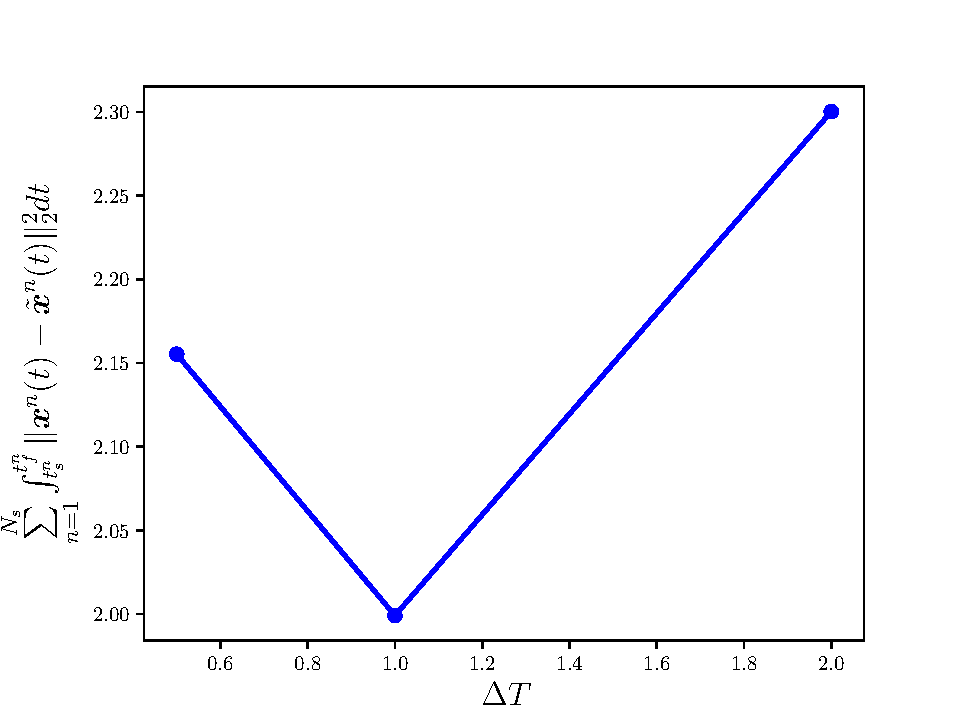
\includegraphics[trim={0cm 0cm 0cm 0cm},clip,width=1.\linewidth]{figs/cavity/error_vs_window_basis2.pdf}
\caption{Integrated $\elltwo$ error}
\label{fig:cav_results2a}
\end{subfigure}
\begin{subfigure}[t]{0.45\textwidth}
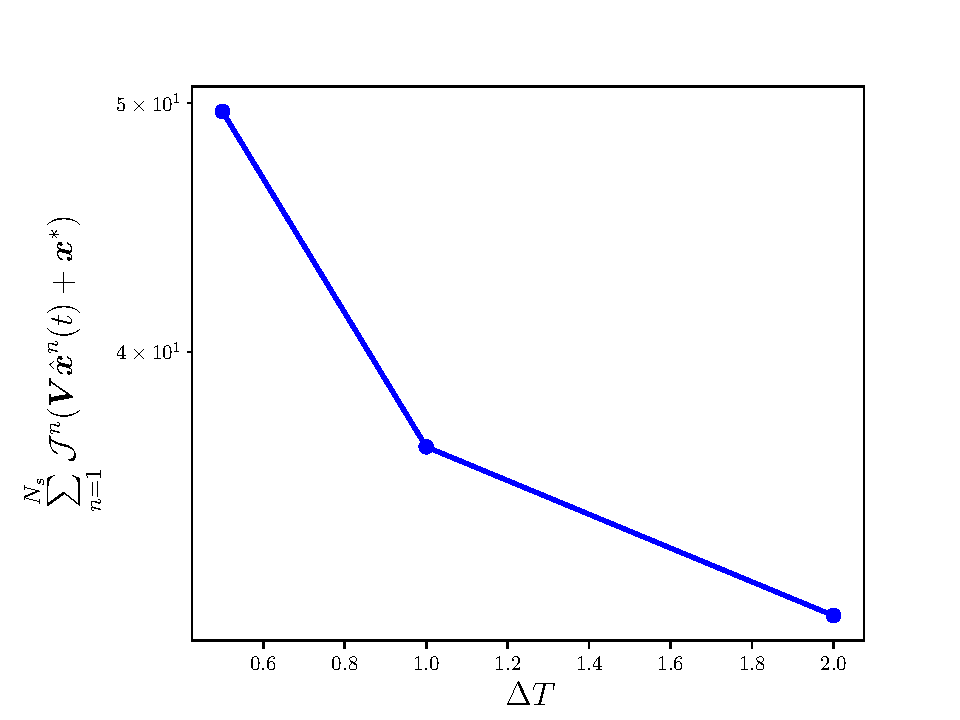
\includegraphics[trim={0cm 0cm 0cm 0cm},clip,width=1.\linewidth]{figs/cavity/objective_vs_window_basis2.pdf}
\caption{Objective function} 
\label{fig:cav_results2b}
\end{subfigure}
\end{center}
\caption{Integrated error (left) and objective function (right) as a function of window size.}
\label{fig:cav_results2}
\end{figure}


\begin{figure}
\begin{center}
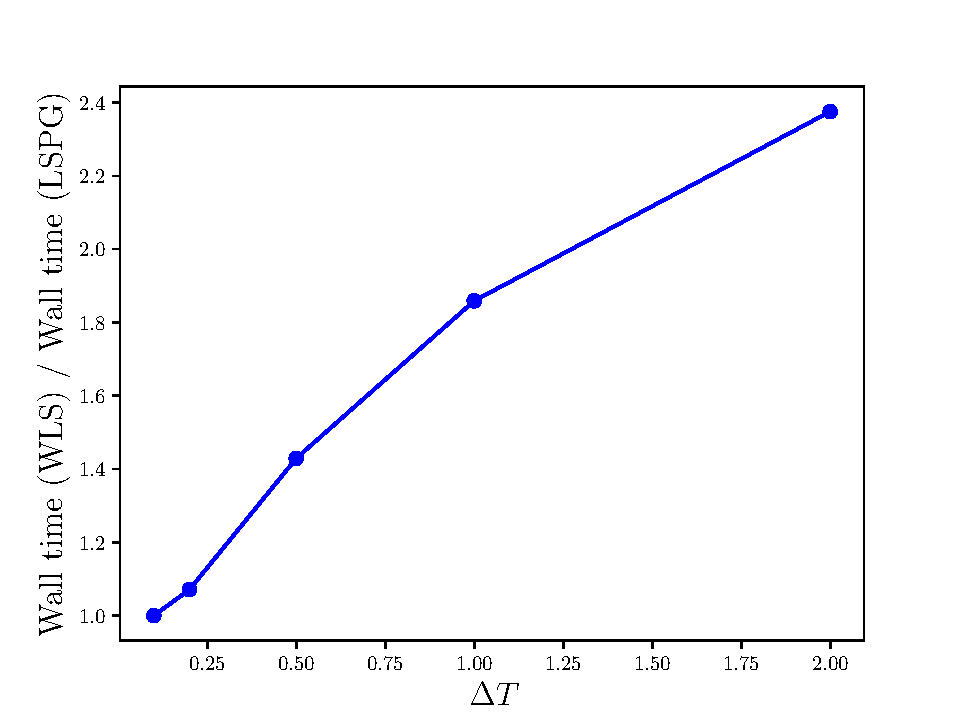
\includegraphics[trim={0cm 0cm 0cm 0cm},clip,width=0.49\linewidth]{figs/cavity/walltime_vs_window_compare_basis2.pdf}
\caption{Wall-clock times of \methodAcronymROMs\ with respect to the LSPG ROM}
\label{fig:cav_wallclock}
\end{center}
\end{figure}

Figure~\ref{fig:cav_snapshots} shows vorticity fields for the FOM, LSPG ROM, and \methodAcronymROM\ with $\Delta T = 0.5$ for the time instance $t = 5.0$. LSPG is observed to exhibit artificial oscillations; the Gauss-Newton method fails to converge at $t \approx 16.0$. The \methodAcronymROM\ at $\Delta T = 0.5$ is able to capture the important features of the flow, including the points of flow separation at the start and end of the ramp, and remains stable for the entire time interval.  

\begin{figure}
\begin{center}
\begin{subfigure}[t]{0.95\textwidth}
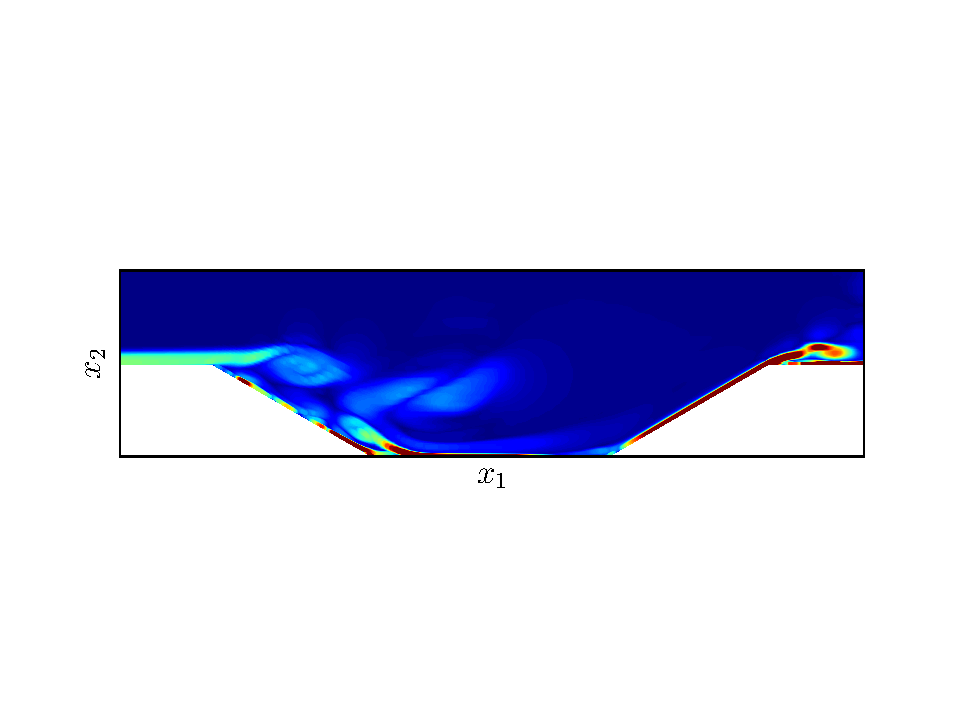
\includegraphics[trim={0cm 3.9cm 0cm 3.9cm},clip,width=1.\linewidth]{figs/cavity/u_fom_t5_basis2.pdf}
\caption{FOM} 
\end{subfigure}
%\begin{subfigure}[t]{0.95\textwidth}
%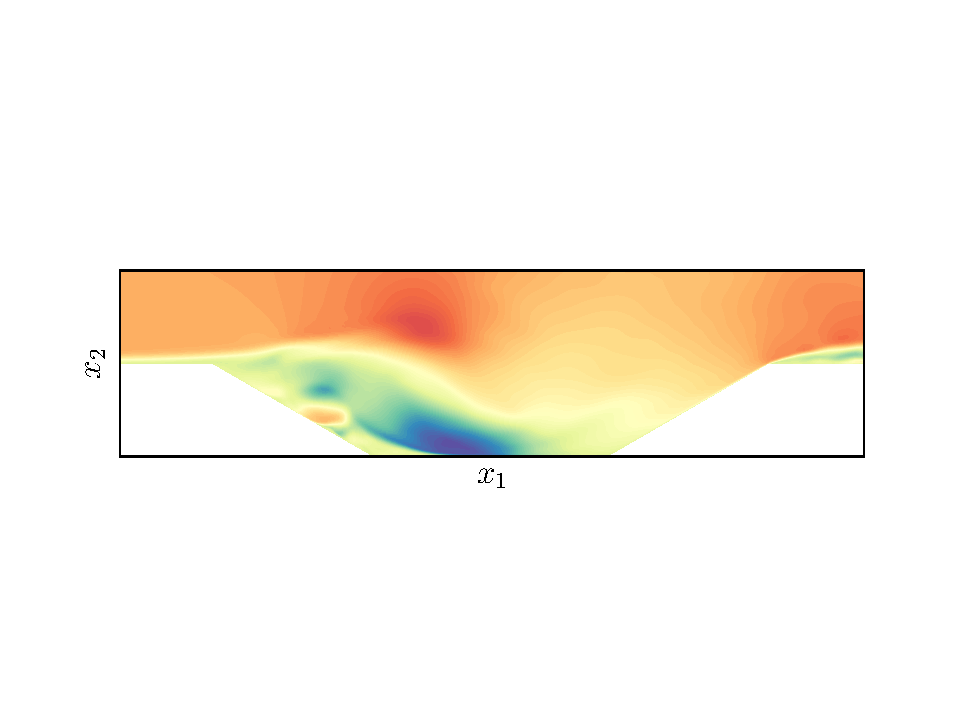
\includegraphics[trim={0cm 3.9cm 0cm 3.9cm},clip,width=1.\linewidth]{figs/cavity/u_c2_t10.pdf}
%\caption{\methodAcronym, $\Delta T = 0.2$} 
%\end{subfigure}
\begin{subfigure}[t]{0.95\textwidth}
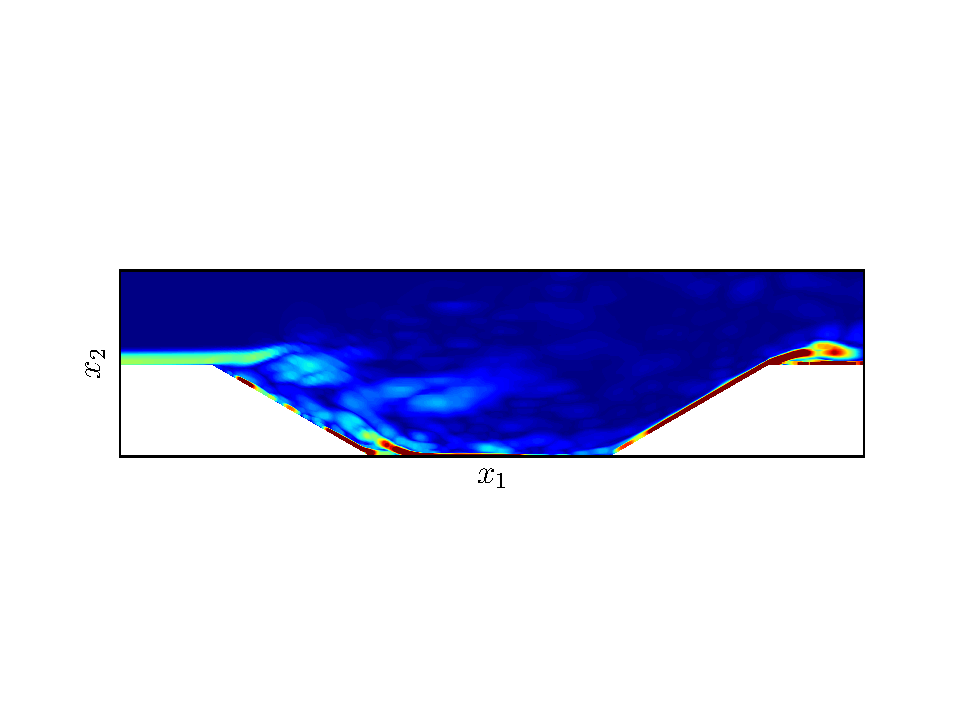
\includegraphics[trim={0cm 3.9cm 0cm 3.9cm},clip,width=1.\linewidth]{figs/cavity/u_lspg_t5_basis2.pdf}
\caption{LSPG} 
\end{subfigure}
\begin{subfigure}[t]{0.95\textwidth}
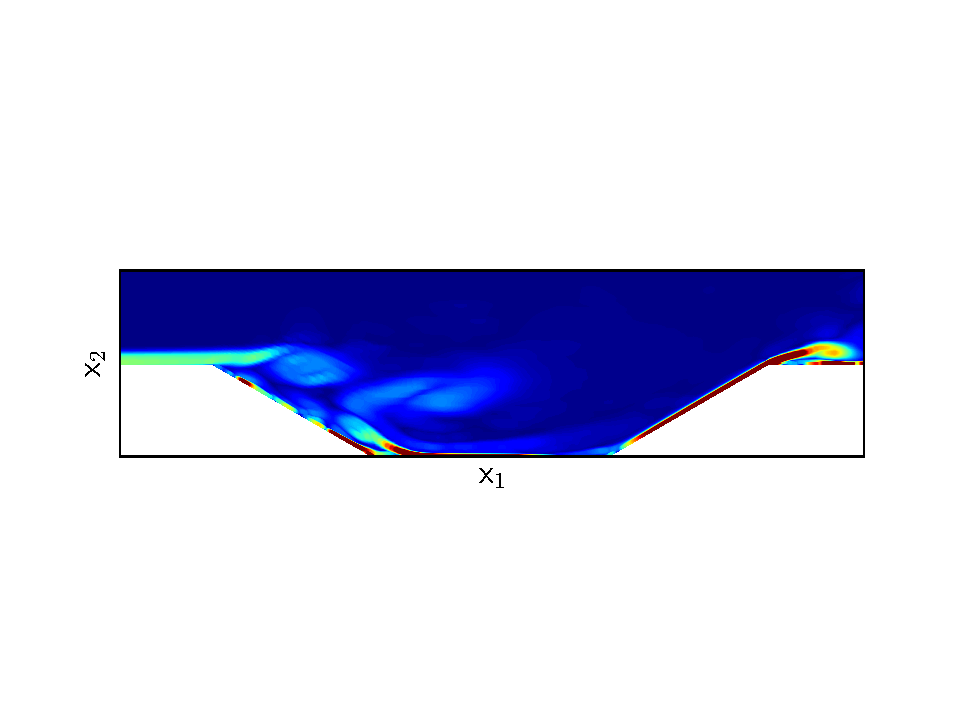
\includegraphics[trim={0cm 3.9cm 0cm 3.9cm},clip,width=1.\linewidth]{figs/cavity/u_c5_t5_basis2.pdf}
\caption{\methodAcronym, $\Delta T = 0.5$} 
\end{subfigure}
%\begin{subfigure}[t]{0.95\textwidth}
%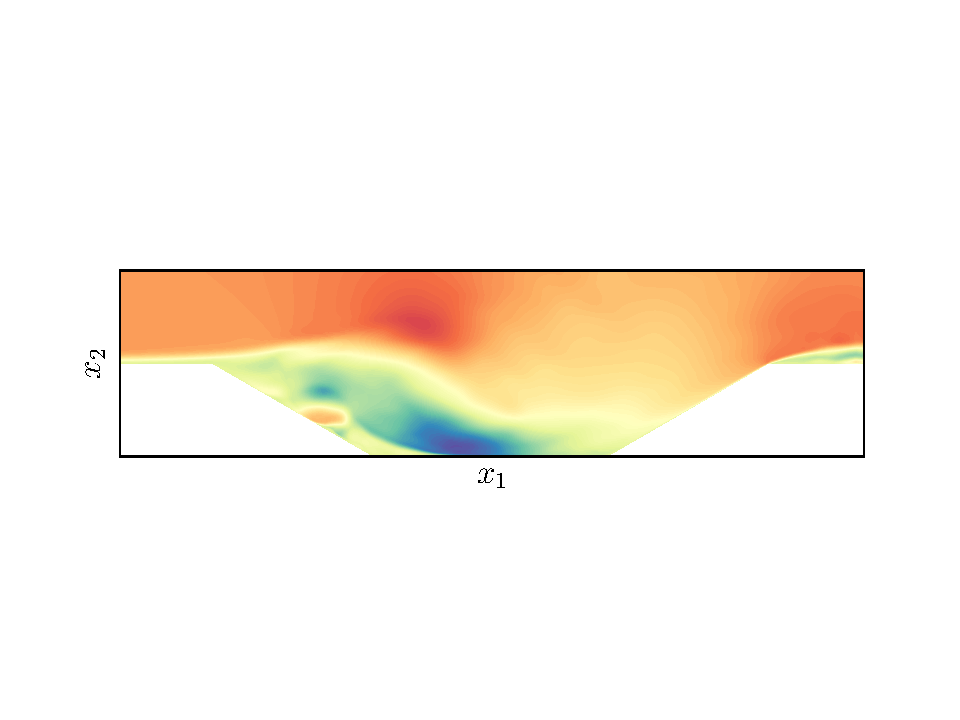
\includegraphics[trim={0cm 3.9cm 0cm 3.9cm},clip,width=1.\linewidth]{figs/cavity/u_c10_t10.pdf}
%\caption{\methodAcronym, $\Delta T = 2.0$} 
%\end{subfigure}
\caption{Field solutions for the vorticity at $t = 5.0$}
\label{fig:cav_snapshots}
\end{center}
\end{figure}


Next, we assess the performance of the various ROMs for basis \#2 as described in Table~\ref{tab:rom_basis_details}, which comprises a richer spatial basis.
 Figure~\ref{fig:cav_results1_basis1} shows the same pressure and error profiles as Figure~\ref{fig:cav_results1}, but for the enriched basis. The LSPG and Galerkin ROMs blow up faster as compared to Figure~\ref{fig:cav_results1}; LSPG fails to converge around $t \approx 8$ (opposed to $t \approx 16$), while Galerkin blows up almost immediately. The 
\methodAcronymROMs\ again yield improved performance: \methodAcronymROMs\ minimizing the residual over window sizes of $\Delta T \ge 0.5$ are seen to all be stable and accurate; the pressure response is well characterized and the normalized state errors are less than $5\%$. The \methodAcronymROMs\ with $\Delta T \ge 0.5$ leveraging the enriched basis yield more accurate results than \methodAcronymROMs\ using the coarse basis.
 

\begin{figure}
\begin{center}

\begin{subfigure}[t]{0.95\textwidth}
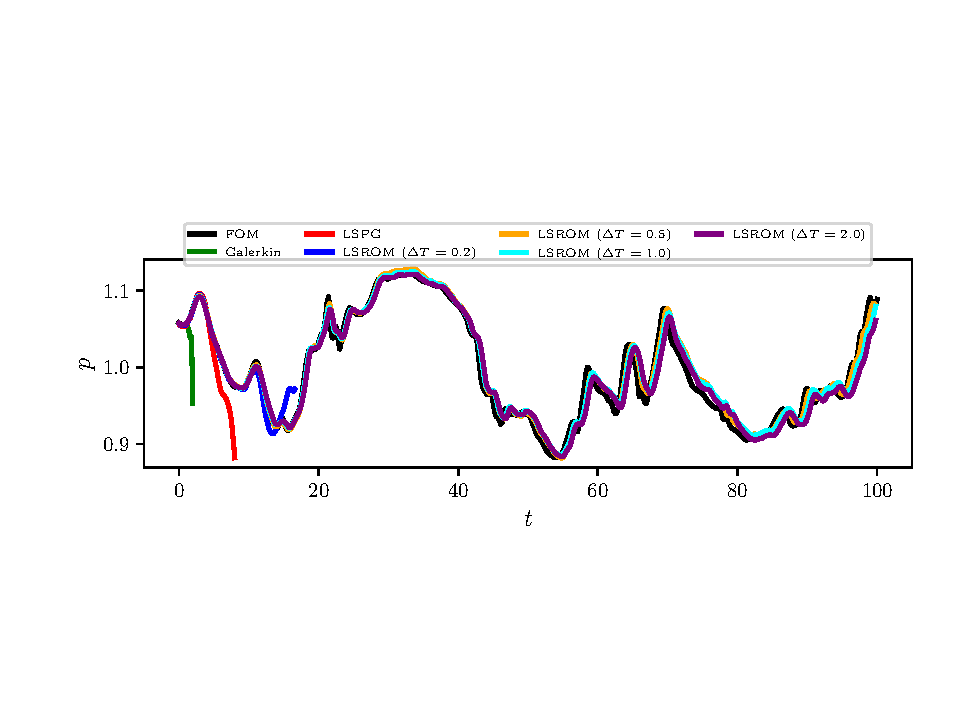
\includegraphics[trim={0cm 2.5cm 0cm 2.5cm},clip,width=1.\linewidth]{figs/cavity/pressure.pdf}
\caption{Pressure} 
\label{fig:cav_results1a_basis1}
\end{subfigure}

\begin{subfigure}[t]{1.0\textwidth}
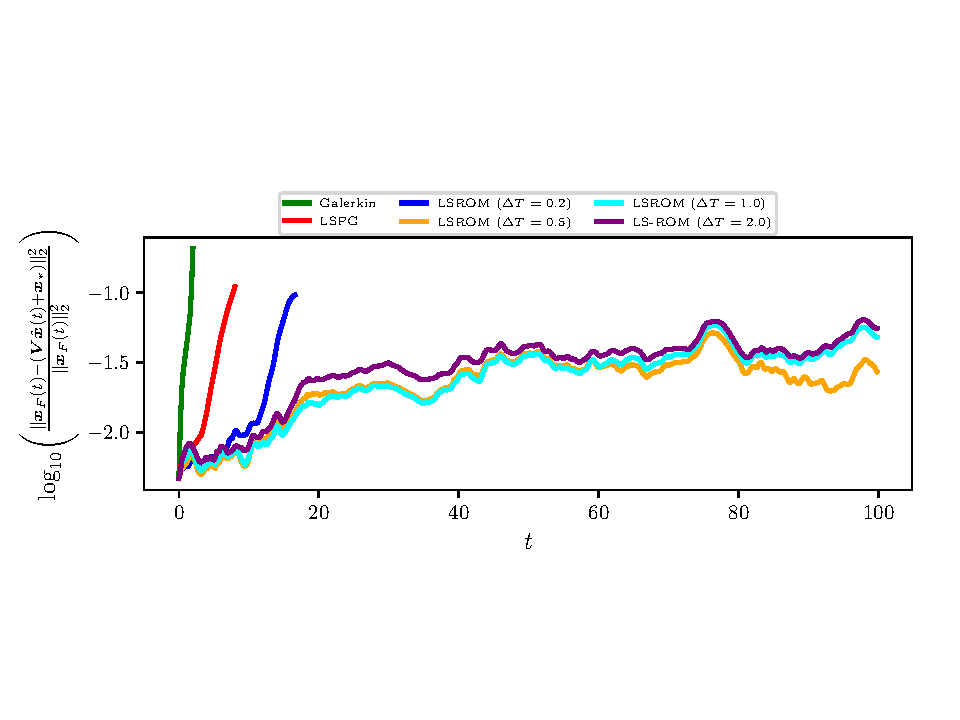
\includegraphics[trim={0cm 2.5cm 0cm 3cm},clip,width=1.\linewidth]{figs/cavity/error.pdf}
\caption{Normalized $\elltwo$ error}
\label{fig:cav_results1b_basis1}
\end{subfigure}
\end{center}
\caption{Comparison of the pressure profiles obtained at the midpoint of the bottom wall (top) and normalized $\elltwo$ state errors (bottom) of various hyper-reduced ROMs to the full-order model solution.}
\label{fig:cav_results1_basis1}
\end{figure}


\begin{figure}
\begin{center}
\begin{subfigure}[t]{0.45\textwidth}
\includegraphics[trim={0cm 0cm 0cm 0cm},clip,width=1.\linewidth]{figs/cavity/error_vs_window.pdf}
\caption{Integrated $\elltwo$ error}
\label{fig:cav_results3a}
\end{subfigure}
\begin{subfigure}[t]{0.45\textwidth}
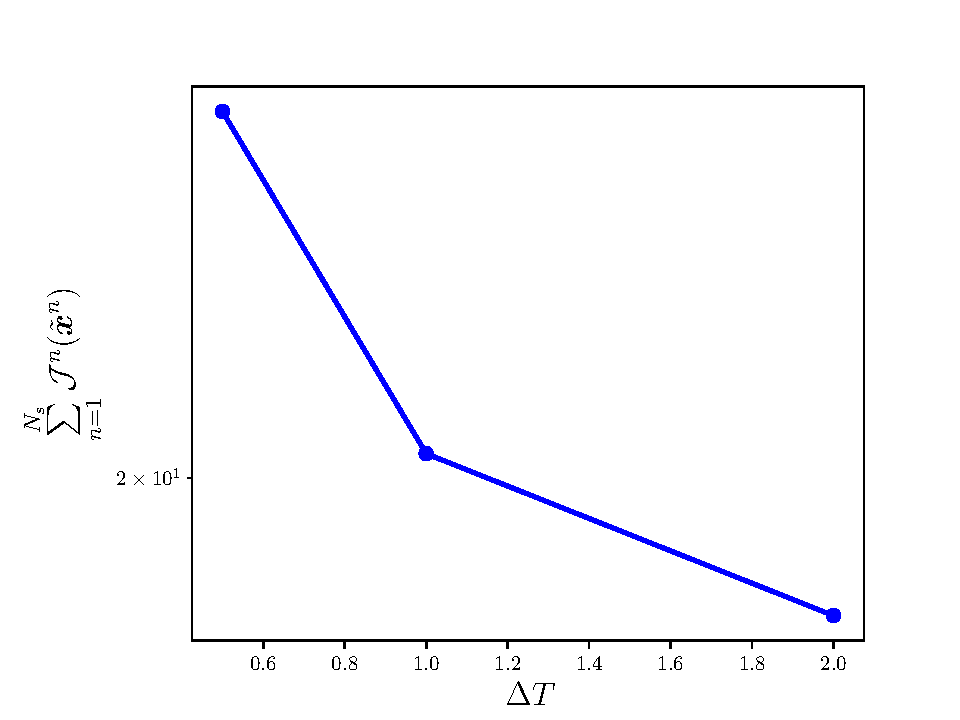
\includegraphics[trim={0cm 0cm 0cm 0cm},clip,width=1.\linewidth]{figs/cavity/objective_vs_window.pdf}
\caption{Objective function} 
\label{fig:cav_results3b}
\end{subfigure}
\end{center}
\caption{Integrated error (left) and objective function (right) as a function of window size.}
\label{fig:cav_results3}
\end{figure}


Finally, Figure~\ref{fig:cav_wallclock} shows the wall-clock times of the \methodAcronymROMs\ as compared to the LSPG ROMs for basis \#2. Increasing the window size again leads to an increase in computational cost. Minimizing the residual over a window comprising 20 time-steps leads to a 2.5x increase in cost over LSPG. This increase in computational cost is particularly reasonable in this example as LSPG yielded an unstable solution. 
\begin{figure}
\begin{center}
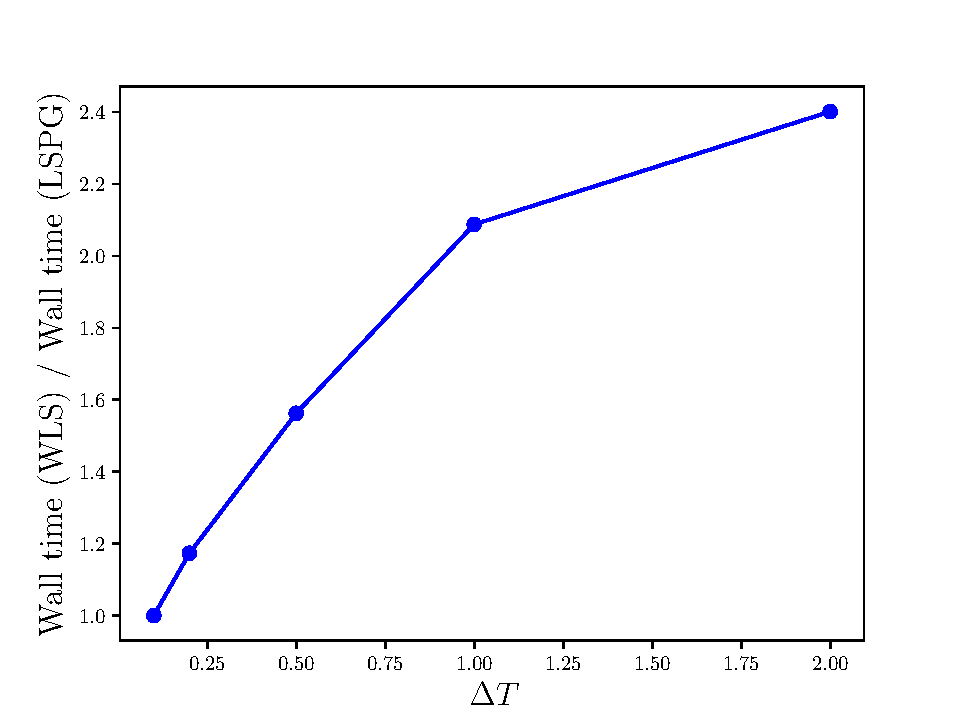
\includegraphics[trim={0cm 0cm 0cm 0cm},clip,width=0.49\linewidth]{figs/cavity/walltime_vs_window_compare.pdf}
\caption{Wall-clock times of \methodAcronymROMs\ with respect to the LSPG ROM.}
\label{fig:cav_wallclock}
\end{center}
\end{figure}


%\begin{figure}
%\begin{center}
%\begin{subfigure}[t]{0.45\textwidth}
%\includegraphics[trim={0cm 0cm 0cm 0cm},clip,width=1.\linewidth]{figs/cavity/error_vs_window.pdf}
%\caption{Integrated $L^2$ error}
%\label{fig:cav_results2a_basis1}
%\end{subfigure}
%\begin{subfigure}[t]{0.45\textwidth}
%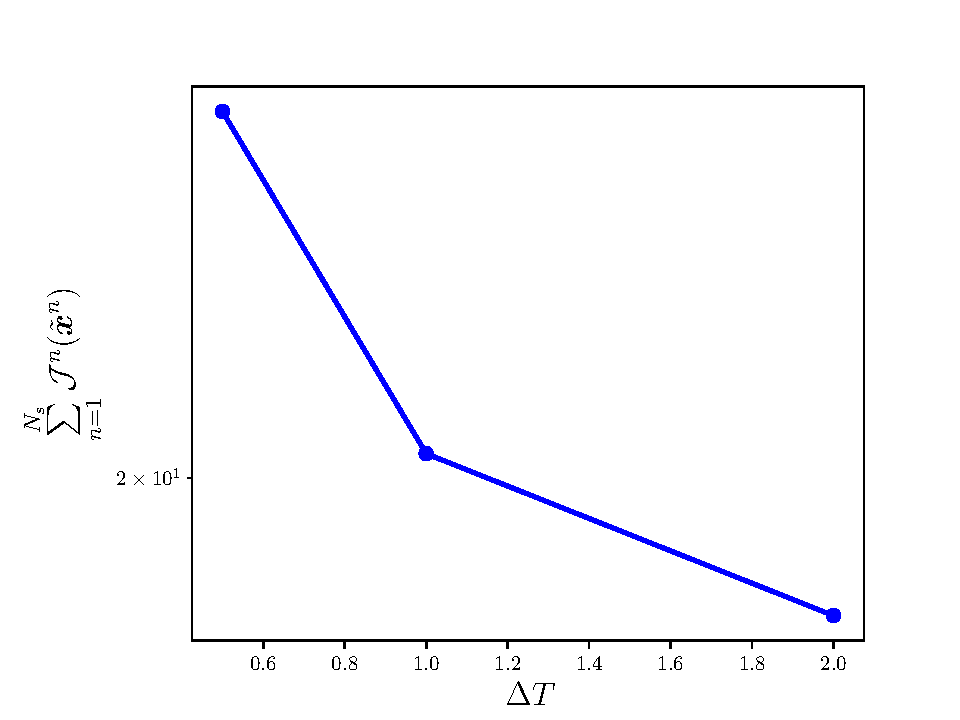
\includegraphics[trim={0cm 0cm 0cm 0cm},clip,width=1.\linewidth]{figs/cavity/objective_vs_window.pdf}
%\caption{Objective function} 
%\label{fig:cav_results2b_basis1}
%\end{subfigure}
%\end{center}
%\caption{Integrated error (left) and objective function (right) as a function of window size.}
%\label{fig:cav_results2_basis1}
%\end{figure}


